% =============================================================================
% CS 552 — Adaptive Drift-Aware Phishing URL Detection
% LaTeX Beamer presentation (implementation & evaluation of Krishnan & Naik 2025)
% Compile: pdflatex -interaction=nonstopmode main.tex  (run twice)
% =============================================================================
\documentclass[aspectratio=169,11pt,xcolor=table]{beamer}

% ----- Packages -----
\usepackage[T1]{fontenc}
\usepackage[utf8]{inputenc}
\usepackage{lmodern}
\usepackage{microtype}
\usepackage{booktabs}
\usepackage{tabularx}
\usepackage{array}
\usepackage{colortbl}
\usepackage{graphicx}
\usepackage{tikz}
\usepackage{pgfplots}
\pgfplotsset{compat=1.18}
\usetikzlibrary{arrows.meta,positioning,calc,shapes.geometric,fit,shadows}
\usepackage{hyperref}
\usepackage{appendixnumberbeamer}
% Note: do NOT load enumitem with Beamer — it breaks \labelenumi grouping.

% ----- Theme / colours (navy academic look; not purple-default) -----
\definecolor{Navy}{HTML}{0B1F3A}
\definecolor{NavyMid}{HTML}{163A63}
\definecolor{Accent}{HTML}{2F6BFF}
\definecolor{AccentSoft}{HTML}{E8F0FF}
\definecolor{Good}{HTML}{0F8A5F}
\definecolor{GoodSoft}{HTML}{E6F7F0}
\definecolor{Warn}{HTML}{B86E00}
\definecolor{WarnSoft}{HTML}{FFF4E0}
\definecolor{Bad}{HTML}{C0392B}
\definecolor{BadSoft}{HTML}{FDECEA}
\definecolor{Muted}{HTML}{5A6A7A}
\definecolor{Rule}{HTML}{D5DEE8}
\definecolor{CardBg}{HTML}{F7F9FC}

\usetheme{default}
\usecolortheme{default}
\setbeamercolor{normal text}{fg=Navy,bg=white}
\setbeamercolor{structure}{fg=Accent}
\setbeamercolor{frametitle}{fg=Navy,bg=white}
\setbeamercolor{title}{fg=white,bg=Navy}
\setbeamercolor{subtitle}{fg=AccentSoft,bg=Navy}
\setbeamercolor{author}{fg=white,bg=Navy}
\setbeamercolor{institute}{fg=AccentSoft,bg=Navy}
\setbeamercolor{date}{fg=AccentSoft,bg=Navy}
\setbeamercolor{block title}{fg=white,bg=NavyMid}
\setbeamercolor{block body}{fg=Navy,bg=CardBg}
\setbeamercolor{block title alerted}{fg=white,bg=Bad}
\setbeamercolor{block body alerted}{fg=Navy,bg=BadSoft}
\setbeamercolor{block title example}{fg=white,bg=Good}
\setbeamercolor{block body example}{fg=Navy,bg=GoodSoft}
\setbeamercolor{itemize item}{fg=Accent}
\setbeamercolor{itemize subitem}{fg=NavyMid}
\setbeamercolor{enumerate item}{fg=Accent}
\setbeamercolor{caption}{fg=Muted}
\setbeamercolor{footline}{fg=Muted,bg=white}
\setbeamercolor{page number in head/foot}{fg=Muted}

\setbeamertemplate{navigation symbols}{}
\setbeamertemplate{itemize items}[circle]
\setbeamertemplate{sections/subsections in toc}[circle]
\setbeamertemplate{frametitle}{%
  \vspace{0.35em}%
  {\usebeamercolor[fg]{frametitle}\Large\bfseries\insertframetitle\par}%
  \vspace{0.15em}%
  {\color{Rule}\hrule height 0.6pt}%
  \vspace{0.55em}%
}
\setbeamertemplate{footline}{%
  \leavevmode%
  \hbox{%
    \begin{beamercolorbox}[wd=.72\paperwidth,ht=2.4ex,dp=1.1ex,left]{footline}%
      \hspace{1.2em}\scriptsize CS\,552 · Krishnan \& Naik, \emph{Security and Privacy} 8(4), e70057 (2025)%
    \end{beamercolorbox}%
    \begin{beamercolorbox}[wd=.28\paperwidth,ht=2.4ex,dp=1.1ex,right]{page number in head/foot}%
      \scriptsize\insertframenumber\hspace{0.15em}/\hspace{0.15em}\inserttotalframenumber\hspace{1.2em}%
    \end{beamercolorbox}%
  }%
  \vskip0pt%
}

% Title page
\setbeamertemplate{title page}{%
  \vspace*{0.4em}
  {\color{AccentSoft}\scriptsize\bfseries CS\,552 · GROUP PROJECT · IMPLEMENTATION \& EVALUATION\par}
  \vspace{0.9em}
  {\LARGE\bfseries\color{white}\inserttitle\par}
  \vspace{0.55em}
  {\large\color{AccentSoft}\insertsubtitle\par}
  \vspace{1.1em}
  {\normalsize\color{white}\insertauthor\par}
  \vspace{0.45em}
  {\small\color{AccentSoft}\insertinstitute\par}
  \vspace{1.2em}
  \begin{tikzpicture}
    \fill[white,opacity=0.08,rounded corners=6pt]
      (0,0) rectangle (\textwidth,2.55);
    \node[anchor=north west,text width=0.62\textwidth,inner sep=10pt]
      at (0.15,2.45) {%
        {\scriptsize\color{Accent}\bfseries ASSIGNED PAPER\par}
        \vspace{0.25em}
        {\footnotesize\color{white}Sruthi Krishnan and Manohar Naik S.
        ``An Efficient Framework for Phishing URL Detection Using Adaptive
        Drift-Aware Feature Monitoring and Online Learning.''
        \emph{Security and Privacy}, 8(4):e70057, 2025.\par}
      };
    \node[anchor=north west,text width=0.28\textwidth,inner sep=10pt]
      at (0.68\textwidth,2.45) {%
        {\scriptsize\color{Accent}\bfseries DOI\par}
        \vspace{0.15em}
        {\footnotesize\color{white}10.1002/spy2.70057\par}
        \vspace{0.55em}
        {\scriptsize\color{Accent}\bfseries JOURNAL\par}
        \vspace{0.15em}
        {\footnotesize\color{white}Wiley · Security \& Privacy\par}
      };
  \end{tikzpicture}
}

% Helpers
\newcommand{\pill}[2][Accent]{%
  \tikz[baseline=(p.base)]\node[fill=#1!15,text=#1!90!black,rounded corners=3pt,
    inner xsep=5pt,inner ysep=1.5pt,font=\scriptsize\bfseries] (p) {#2};%
}
\newcommand{\kpi}[3][Accent]{%
  \begin{tikzpicture}
    \node[draw=Rule,fill=CardBg,rounded corners=5pt,inner sep=7pt,
      text width=\linewidth-14pt,align=center] {%
      {\scriptsize\color{Muted}#2\par}
      \vspace{0.15em}
      {\Large\bfseries\color{#1}#3\par}
    };
  \end{tikzpicture}%
}
\newcommand{\tagline}[1]{%
  \begin{tikzpicture}
    \node[fill=Navy,text=white,rounded corners=5pt,inner sep=8pt,
      text width=\linewidth-16pt,align=left,font=\small] {#1};
  \end{tikzpicture}%
}
\newcommand{\capnote}[1]{{\scriptsize\color{Muted}#1\par}}

\title{An Efficient Framework for Phishing URL Detection\\Using Adaptive Drift-Aware Feature Monitoring and Online Learning}
\subtitle{Implementation and evaluation of Krishnan \& Naik (2025)}
\author{Pratham Garg \quad·\quad Sumit Sharma \quad·\quad Vivaan Garg}
\institute{CS\,552 Group Project}
\date{}

\begin{document}

% =============================================================================
\begin{frame}[plain]
  \begin{tikzpicture}[remember picture,overlay]
    \fill[Navy] (current page.south west) rectangle (current page.north east);
  \end{tikzpicture}
  \vspace*{0.6em}
  \titlepage
\end{frame}

% =============================================================================
\begin{frame}{Roadmap: from ``why?'' to ``does it work?''}
\begin{columns}[T,onlytextwidth]
\begin{column}{0.19\textwidth}
  \begin{block}{1 · Problem}
  \scriptsize Phishing links \& concept drift
  \end{block}
\end{column}
\begin{column}{0.19\textwidth}
  \begin{block}{2 · Idea}
  \scriptsize Watch drift, re-pick features, learn online
  \end{block}
\end{column}
\begin{column}{0.19\textwidth}
  \begin{exampleblock}{3 · How}
  \scriptsize Features → LASSO+MI → SGD → KS → loop
  \end{exampleblock}
\end{column}
\begin{column}{0.19\textwidth}
  \begin{block}{4 · Build}
  \scriptsize \texttt{drift\_phish}, data, 5 experiments
  \end{block}
\end{column}
\begin{column}{0.19\textwidth}
  \begin{alertblock}{5 · Results}
  \scriptsize What reproduced --- and what did not
  \end{alertblock}
\end{column}
\end{columns}
\vspace{0.7em}
\tagline{A phishing detector that \textbf{notices when attackers change style},
re-picks the most useful clues, and \textbf{keeps learning in milliseconds}
instead of retraining from scratch.}
\end{frame}

% =============================================================================
\begin{frame}{Phishing starts with a link that looks almost right}
\begin{columns}[T,onlytextwidth]
\begin{column}{0.55\textwidth}
  \begin{exampleblock}{Real}
  \texttt{\footnotesize https://www.paypal.com/signin}
  \end{exampleblock}
  \vspace{0.35em}
  \begin{alertblock}{Phishing}
  \texttt{\footnotesize http://secure-paypal-login.\textbf{tk}/confirm/...}
  \end{alertblock}
  \vspace{0.45em}
  \begin{block}{Why this is hard}
  \small Blocklists lag brand-new links. We need a model that judges a URL
  \textbf{it has never seen} --- from the URL string alone.
  \end{block}
\end{column}
\begin{column}{0.42\textwidth}
  \renewcommand{\arraystretch}{1.25}
  {\footnotesize
  \begin{tabular}{@{}lcc@{}}
  \toprule
  & Page content & \textbf{URL-only} \\
  \midrule
  Needs & download page & URL text \\
  Speed & slow & instant \\
  Privacy & reads page & no page read \\
  Safety & visits site & never visits \\
  \bottomrule
  \end{tabular}}
  \vspace{0.7em}
  \tagline{\textbf{Key question:} can URL text alone stay accurate as attacks evolve?}
\end{column}
\end{columns}
\end{frame}

% =============================================================================
\begin{frame}{The catch: a model trained once goes stale (concept drift)}
\begin{columns}[T,onlytextwidth]
\begin{column}{0.48\textwidth}
  \begin{block}{What is concept drift?}
  \small Statistics of phishing URLs \textbf{change over time} --- shorter hostnames,
  more random characters, fewer bait words. Yesterday's model errs on today's URLs.
  \end{block}
  \vspace{0.4em}
  \begin{alertblock}{We measured it}
  \small \textbf{34 of 58} features shift (KS, $\delta{=}0.05$) between old corpora
  and PhishTank Jun\,2024--Jan\,2025.
  \end{alertblock}
  \vspace{0.4em}
  \begin{block}{Obvious fix is expensive}
  \small Full retrain $\approx$ \textbf{4\,s} on 210k URLs vs \textbf{1.5\,ms} incremental update.
  \end{block}
\end{column}
\begin{column}{0.49\textwidth}
  \centering
  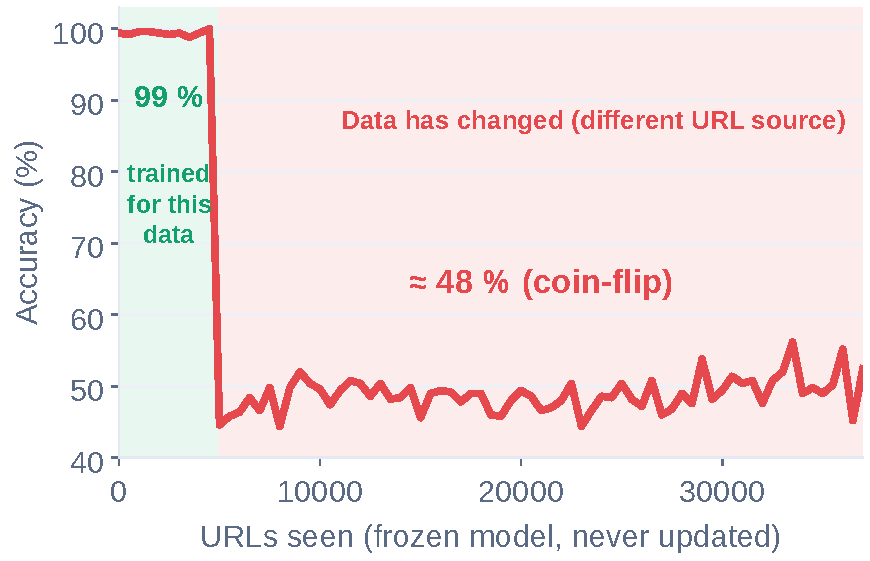
\includegraphics[width=\linewidth]{figures/c_frozen_decay.pdf}\\[0.3em]
  \capnote{S2: frozen model scores \textbf{99\%} on its train domain, then $\approx$\textbf{48\%}
  (coin-flip) after the URL source changes.}
\end{column}
\end{columns}
\end{frame}

% =============================================================================
\begin{frame}{Paper idea: three ingredients that stay current}
\begin{columns}[T,onlytextwidth]
\begin{column}{0.52\textwidth}
  \centering
  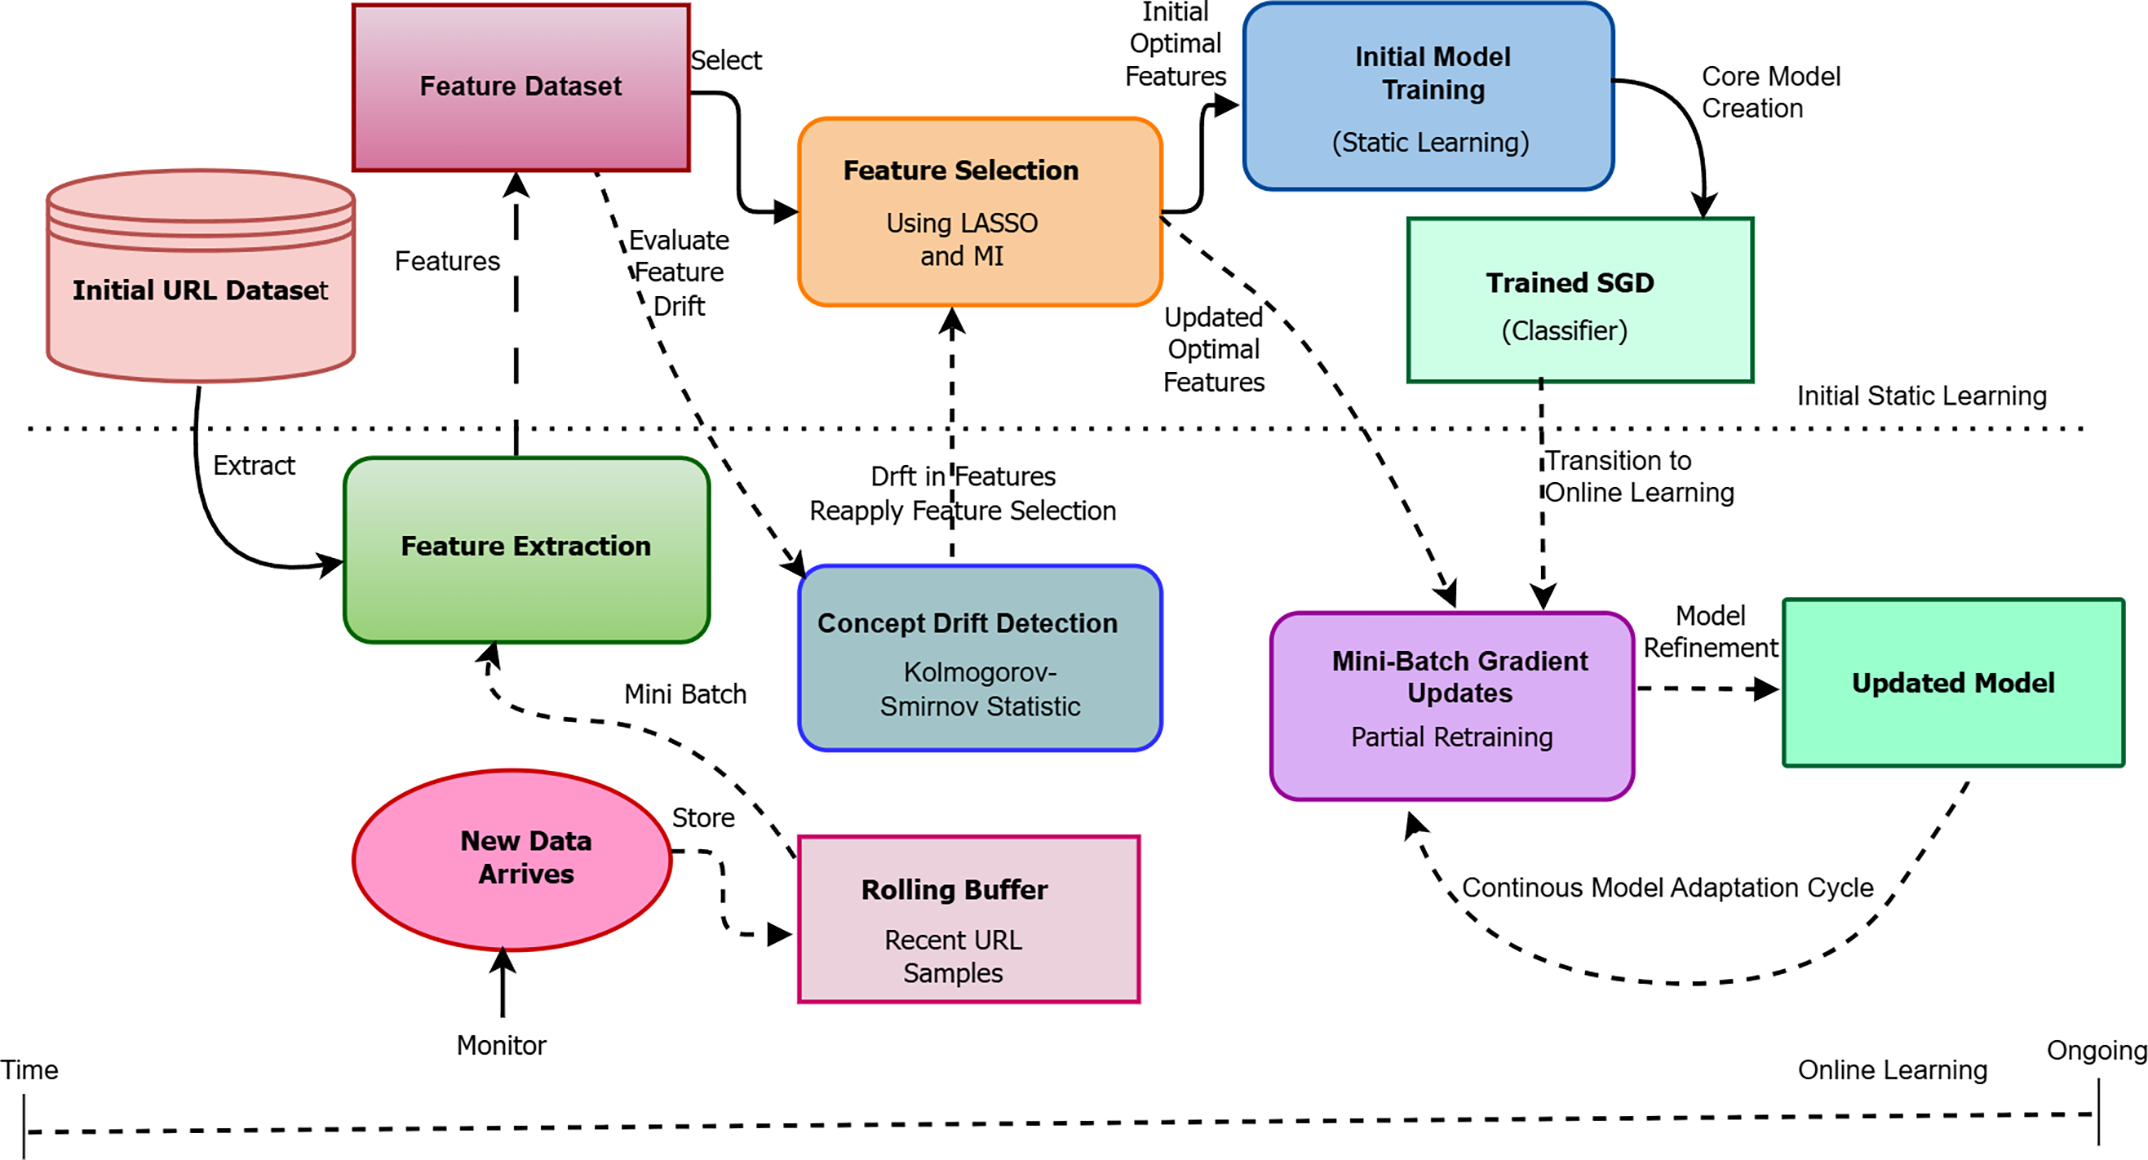
\includegraphics[width=\linewidth]{figures/paper_fig1_arch.png}\\[0.25em]
  \capnote{Paper Fig.\,1: offline once (top); online forever (bottom).}
\end{column}
\begin{column}{0.45\textwidth}
  \begin{enumerate}
    \item \textbf{Pick best clues} --- LASSO + mutual information; keep top quartile $F^*$.
    \item \textbf{Watch for change} --- Kolmogorov--Smirnov test per feature vs.\ history.
    \item \textbf{Learn on the fly} --- online SGD mini-batches; no full retrain.
  \end{enumerate}
  \vspace{0.55em}
  \begin{exampleblock}{Paper headline claim}
  \centering\textbf{99.85\%} accuracy · \textbf{0.067\%} FPR
  \end{exampleblock}
\end{column}
\end{columns}
\end{frame}

% =============================================================================
\begin{frame}{Our task: implement every box of Fig.\,1}
\small
\begin{block}{Assignment}
Implement the paper's methodology and reproduce experiments. Package
\texttt{drift\_phish} ($\sim$1{,}200 LOC) + 5 experiment scripts + 16 unit tests + browser demo.
\end{block}
\vspace{0.35em}
\renewcommand{\arraystretch}{1.2}
\begin{tabular}{@{}llll@{}}
\toprule
\textbf{Paper box} & \textbf{Module} & \textbf{Key knobs} \\
\midrule
URL $\to$ features & \texttt{features/extractor.py} & 58 lexical features \\
Feature selection & \texttt{selection/dynamic.py} & $S{=}w{+}I$, $\tau{=}P_{75}$ \\
SGD classifier & \texttt{learning/online\_sgd.py} & $\eta_0{=}0.01$, balanced \\
Drift detection & \texttt{drift/ks\_monitor.py} & $\delta{=}0.05$, buf 1500 \\
Online loop & \texttt{framework.py} & $B{=}500$, adaptive mode \\
\bottomrule
\end{tabular}
\vspace{0.45em}
\tagline{Modes for fair comparison: \textbf{adaptive} (proposed) ·
\textbf{online\_static} · \textbf{frozen} · \textbf{periodic\_batch}.
One command: \texttt{make all}.}
\end{frame}

% =============================================================================
\begin{frame}{Step 1 --- Turning a URL into numbers}
\small
\begin{center}
{\ttfamily\footnotesize
\textcolor{Warn}{http://}\textcolor{Accent}{secure-paypal-login}\textcolor{Bad}{.tk}%
\textcolor{Good}{/confirm/account}\textcolor{NavyMid}{?user=1\&id=88}}
\end{center}
\vspace{0.3em}
\renewcommand{\arraystretch}{1.15}
\begin{columns}[T,onlytextwidth]
\begin{column}{0.62\textwidth}
{\footnotesize
\begin{tabular}{@{}lrr@{}}
\toprule
Feature & wikipedia.org & phishing URL \\
\midrule
\texttt{url\_length} & 39 & \textbf{58} \\
\texttt{num\_hyphens} & 0 & \textbf{2} \\
\texttt{number\_count} & 0 & \textbf{3} \\
\texttt{entropy} & 3.78 & \textbf{4.62} \\
\texttt{has\_https} / \texttt{scheme\_http} & 1 / 0 & \textbf{0 / 1} \\
\texttt{suspicious\_tld} & 0 & \textbf{1} \\
\texttt{suspicious\_term\_frequency} & 0 & \textbf{4} \\
\bottomrule
\end{tabular}}
\end{column}
\begin{column}{0.35\textwidth}
  \begin{exampleblock}{Result}
  Each URL $\to$ \textbf{58 numbers}. Pure string processing $\approx$ \textbf{0.16\,ms}/URL --- no download.
  \end{exampleblock}
\end{column}
\end{columns}
\end{frame}

% =============================================================================
\begin{frame}{58 URL clues in six families (paper Table 3)}
\begin{columns}[T,onlytextwidth]
\begin{column}{0.32\textwidth}
  \begin{block}{Length \& size · 8}
  \scriptsize url / domain / path / query length, tokens, \ldots
  \end{block}
  \vspace{0.25em}
  \begin{block}{Digits \& randomness · 6}
  \scriptsize number\_count, digit\_ratio, entropy, host\_entropy
  \end{block}
\end{column}
\begin{column}{0.32\textwidth}
  \begin{block}{Structure \& symbols · 18}
  \scriptsize dots, slashes, hyphens, \texttt{=}, \texttt{\&}, \texttt{@}, \texttt{\%}
  \end{block}
  \vspace{0.25em}
  \begin{alertblock}{Bait \& brands · 11}
  \scriptsize login, verify, secure, free, brand proximity
  \end{alertblock}
\end{column}
\begin{column}{0.32\textwidth}
  \begin{block}{Obfuscation · 9}
  \scriptsize IP host, shorteners, suspicious TLD, homoglyphs
  \end{block}
  \vspace{0.25em}
  \begin{exampleblock}{Scheme \& redirects · 6}
  \scriptsize https/http; redirect \& domain-mismatch = \textbf{lexical proxies}
  \end{exampleblock}
\end{column}
\end{columns}
\vspace{0.55em}
\begin{block}{Honest note}
\small Paper's redirect-chain / domain-mismatch need live HTTP. We use lexical proxies
(e.g.\ contains \texttt{redirect=} or a second \texttt{http}) so everything stays URL-string-only.
\end{block}
\end{frame}

% =============================================================================
\begin{frame}{Step 2 --- Not every clue helps: keep the top quarter}
\begin{columns}[T,onlytextwidth]
\begin{column}{0.48\textwidth}
  \centering
  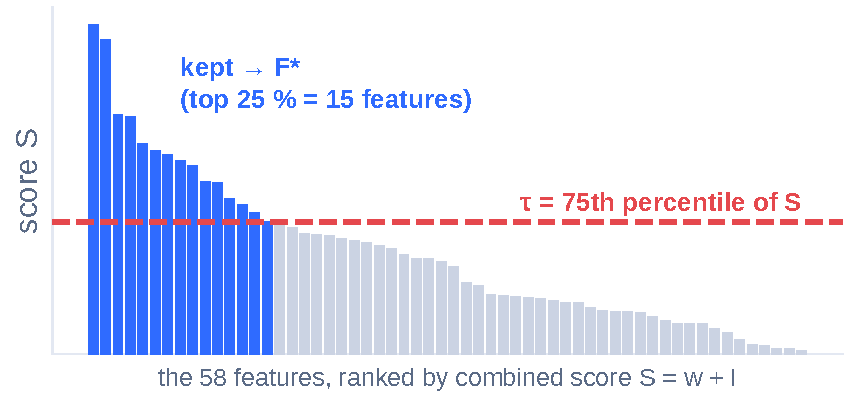
\includegraphics[width=0.95\linewidth]{figures/i_selection.pdf}\\[0.2em]
  \capnote{Rank 58 features by $S$; top quartile (blue) = active set $F^*$.}
\end{column}
\begin{column}{0.49\textwidth}
  \small
  \begin{enumerate}
    \item \textbf{LASSO} ($\lambda{=}10^{-4}$) $\to$ weights $w$ (useless $\to 0$)
    \item \textbf{Mutual information} $\to$ scores $I$ (also non-linear clues)
    \item Combined score $S = w + I$
    \item Keep $S \ge \tau$, $\tau = P_{75}(S)$ $\Rightarrow$ $|F^*|{=}15$
  \end{enumerate}
  \vspace{0.35em}
  \begin{block}{Why shrink \& re-select?}
  Faster, less overfitting, interpretable. Best clues \textbf{change} when attackers change tactics.
  \end{block}
\end{column}
\end{columns}
\end{frame}

% =============================================================================
\begin{frame}{Step 3 --- Linear SVM + SGD: draw a line, then nudge it}
\begin{columns}[T,onlytextwidth]
\begin{column}{0.52\textwidth}
  \centering
  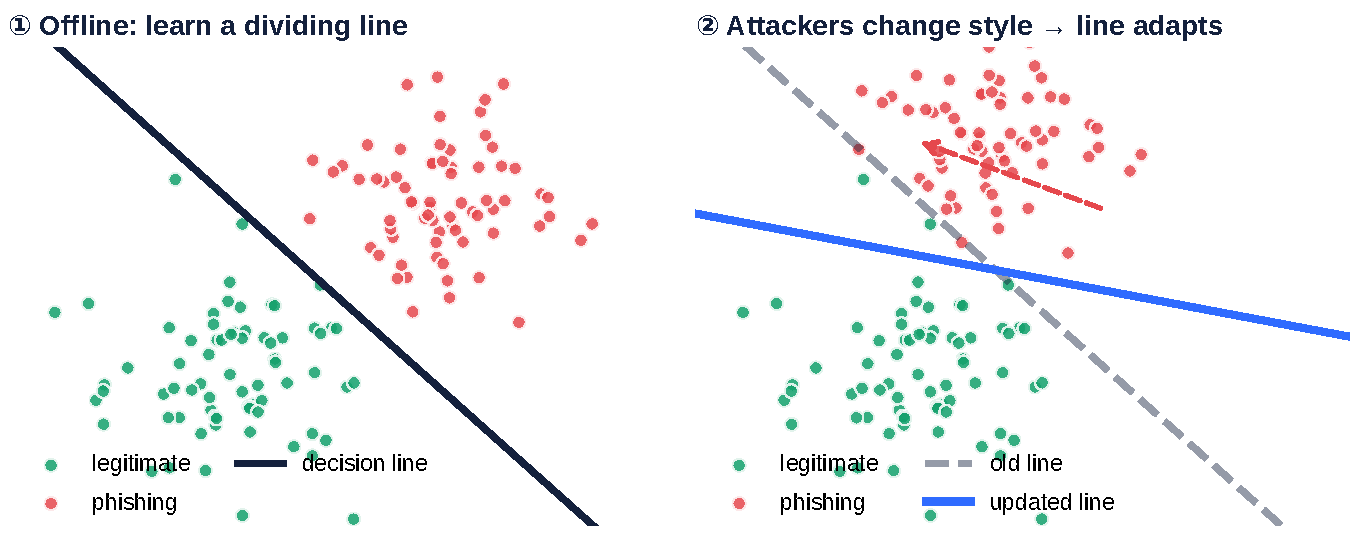
\includegraphics[width=\linewidth]{figures/i_boundary.pdf}\\[0.2em]
  \capnote{Offline: separate legit vs phishing. Online: mini-batch updates tilt the line.}
\end{column}
\begin{column}{0.45\textwidth}
  \begin{block}{Why SGD?}
  \small Learns from \textbf{small chunks} --- \texttt{partial\_fit} on a 500-URL batch instead of re-reading the whole corpus.
  \end{block}
  \vspace{0.35em}
  \small Variants: \pill{SGD-SVM ★} \pill[Warn]{SGD-LR} \pill[Good]{SGD-Perceptron}
  \vspace{0.45em}
  \begin{block}{Table 4 knobs we used}
  \scriptsize $\eta_0{=}0.01$ · adaptive LR · balanced · early stop ·
  buffer 1500 · $B{=}500$ · KS $\delta{=}0.05$ · 80:20 · seed 42
  \end{block}
\end{column}
\end{columns}
\end{frame}

% =============================================================================
\begin{frame}{Step 4 --- KS test: ``do these two samples look alike?''}
\begin{columns}[T,onlytextwidth]
\begin{column}{0.5\textwidth}
  \centering
  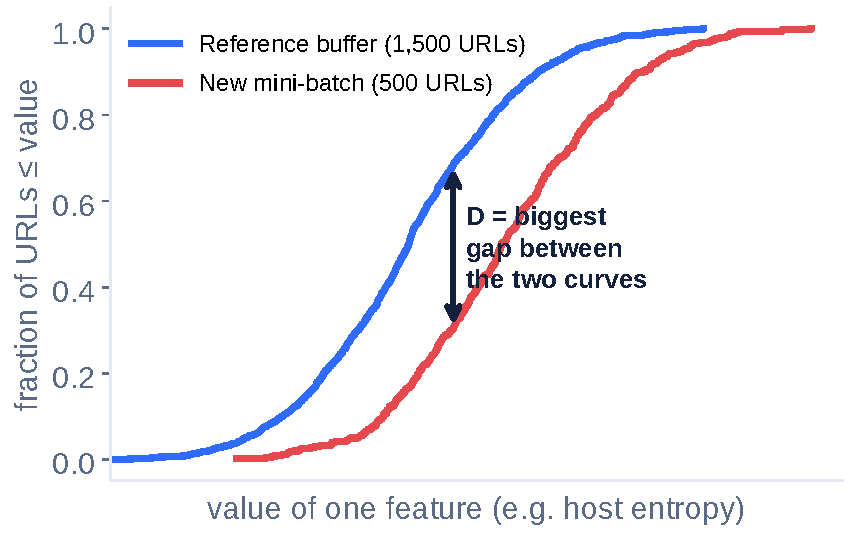
\includegraphics[width=\linewidth]{figures/i_ks.pdf}\\[0.2em]
  \capnote{$D$ = largest vertical gap between reference CDF and new-batch CDF.}
\end{column}
\begin{column}{0.47\textwidth}
  \begin{enumerate}
    \item Reference = last \textbf{1{,}500} labelled URLs
    \item Every mini-batch $B{=}500$: KS per feature
    \item $p < \delta{=}0.05$ $\Rightarrow$ that feature drifted
  \end{enumerate}
  \vspace{0.45em}
  \begin{alertblock}{Paper leaves the event rule open}
  \small \textbf{Our rule:} drift event when $\ge$\textbf{25\%} of active features $F^*$ fail KS.
  \end{alertblock}
\end{column}
\end{columns}
\end{frame}

% =============================================================================
\begin{frame}{Step 5 --- The online loop (every mini-batch)}
\small
\begin{center}
\pill[Muted]{500 URLs}
\;$\to$\;
\pill{1 Predict}
\;$\to$\;
\pill[Warn]{2 KS test}
\;$\to$\;
\pill[Bad]{3 Drift?}
\;$\to$\;
\pill[Good]{4 Learn (partial\_fit)}
\end{center}
\vspace{0.4em}
\begin{columns}[T,onlytextwidth]
\begin{column}{0.62\textwidth}
  \begin{alertblock}{If drift is detected}
  \begin{enumerate}
    \item Mark drifted features in $F^*$ obsolete
    \item Re-run LASSO+MI on the buffer
    \item Blend with importance history $H$ (50/50)
    \item New $F^*$ = top quartile again
    \item Mask removed features; 3 replay epochs
    \item Reset KS reference to the new buffer
  \end{enumerate}
  \end{alertblock}
\end{column}
\begin{column}{0.35\textwidth}
  \begin{block}{Why predict first?}
  Prequential evaluation: every URL scored by a model that has \textbf{not} seen it yet.
  \end{block}
\end{column}
\end{columns}
\end{frame}

% =============================================================================
\begin{frame}{Data and the five experiments}
\begin{columns}[T,onlytextwidth]
\begin{column}{0.55\textwidth}
{\footnotesize
\begin{tabular}{@{}lrl@{}}
\toprule
Corpus & URLs & Role \\
\midrule
PhiUSIIL & 235k & Table 7 \\
Kaggle subset & 21k & Table 6 \\
ISCX-URL-2016 & 15.4k & Table 5 (79 feats) \\
Hannousse 2021 & 11.4k & raw URLs (ISCX stand-in) \\
Combined & 263k & Fig.\,6 \\
\textbf{PhishTank stream} & 12{,}888 & Jun\,24--Jan\,25 \\
\bottomrule
\end{tabular}}
\end{column}
\begin{column}{0.42\textwidth}
  \small
  \begin{enumerate}
    \item Offline (T5--7, Fig.\,6)
    \item Online streams S1 / S2
    \item Ablation (Table 9)
    \item Runtime (T10--11)
    \item Drift analysis (Figs.\,4,5,7; T8)
  \end{enumerate}
\end{column}
\end{columns}
\vspace{0.5em}
\begin{block}{Setup}
\small Positive = phishing · 80:20 seed 42 · streams: 5 seeds (mean$\pm$std) · $B{=}500$.
\end{block}
\end{frame}

% =============================================================================
\begin{frame}{Results 1 --- Offline: SGD-SVM best linear model}
\begin{columns}[T,onlytextwidth]
\begin{column}{0.52\textwidth}
  \centering
  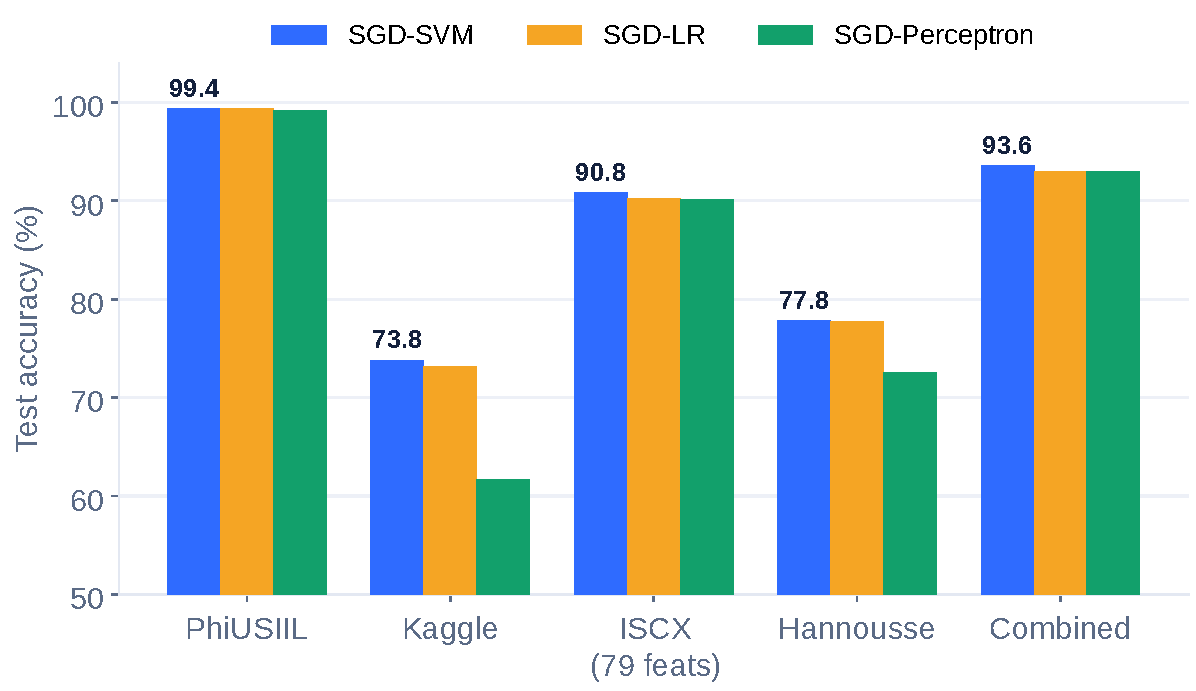
\includegraphics[width=\linewidth]{figures/c_offline_variants.pdf}\\[0.15em]
  \capnote{Our Fig.\,6 analogue: SVM best or tied on every corpus.}
\end{column}
\begin{column}{0.45\textwidth}
{\footnotesize
\begin{tabular}{@{}lrrr@{}}
\toprule
Corpus & Ours & Paper & \\
\midrule
PhiUSIIL & \textbf{99.38} & 98.78 & \textcolor{Good}{\checkmark} \\
ISCX & 90.83 & 99.02 & $\approx$ \\
Kaggle & 73.81 & 99.00 & $\approx$ \\
Combined & 93.58 & 99.85 & $\approx$ \\
\bottomrule
\end{tabular}}
  \vspace{0.45em}
  \begin{exampleblock}{PhiUSIIL highlight}
  \centering\textbf{99.38\%} acc · FPR \textbf{0.004\%}
  \end{exampleblock}
  \vspace{0.3em}
  {\scriptsize\color{Muted}$\approx$ = same method ordering, lower absolute level.}
\end{column}
\end{columns}
\end{frame}

% =============================================================================
\begin{frame}{Why Kaggle / ISCX / combined numbers are lower}
\begin{columns}[T,onlytextwidth]
\begin{column}{0.5\textwidth}
  \centering
  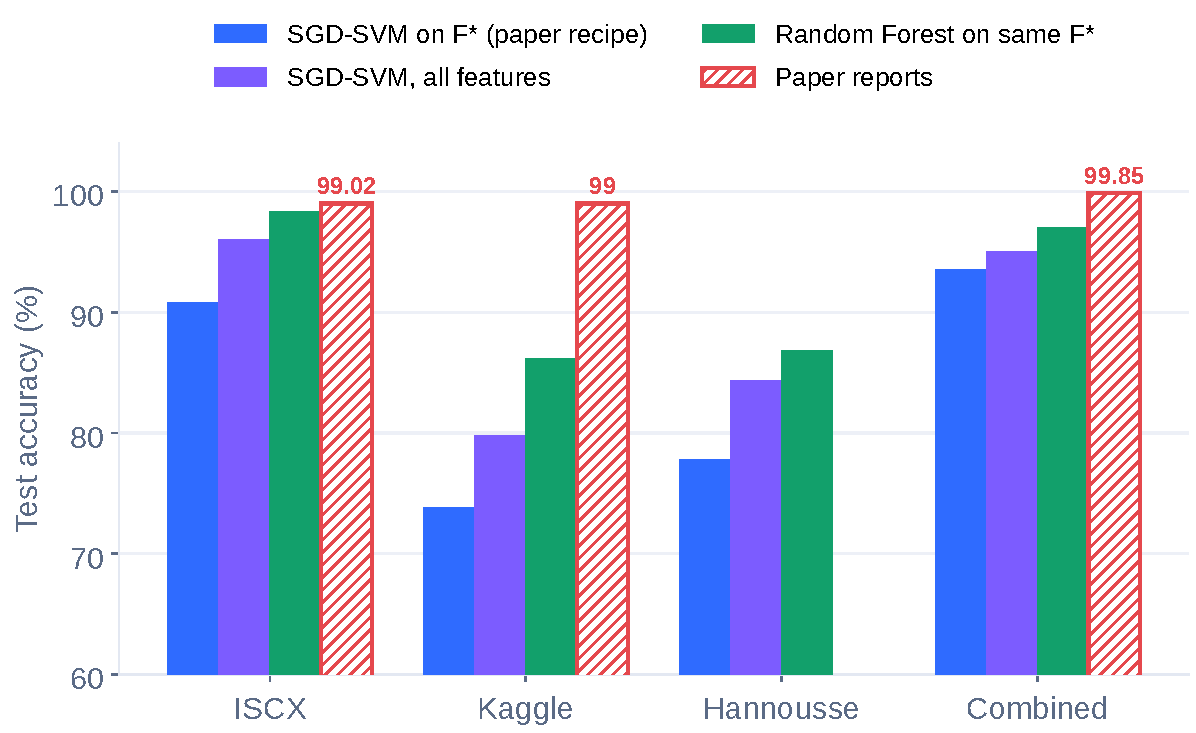
\includegraphics[width=\linewidth]{figures/c_gap.pdf}\\[0.15em]
  \capnote{All-features lifts ISCX 90.8$\to$96.1\%; RF on same $F^*$ reaches 98.3\%.}
\end{column}
\begin{column}{0.47\textwidth}
  \begin{enumerate}
    \item \textbf{Feature set:} only top-quartile $F^*$; paper does not publish exact defs.
    \item \textbf{Data versions:} no published cleaning / versions; ISCX only as vectors.
    \item \textbf{Corpora differ:} PhiUSIIL benign mostly bare domains (easy); Kaggle/Hannousse much harder.
  \end{enumerate}
  \vspace{0.4em}
  \centering
  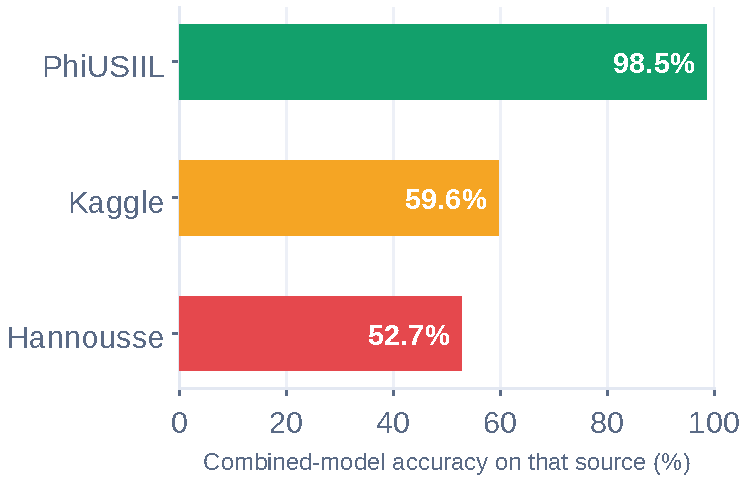
\includegraphics[width=0.85\linewidth]{figures/c_per_source.pdf}
\end{column}
\end{columns}
\end{frame}

% =============================================================================
\begin{frame}{Results 2 --- Drift is real: old vs new phishing}
\begin{columns}[T,onlytextwidth]
\begin{column}{0.38\textwidth}
  \centering
  {\scriptsize Paper Fig.\,4}\\
  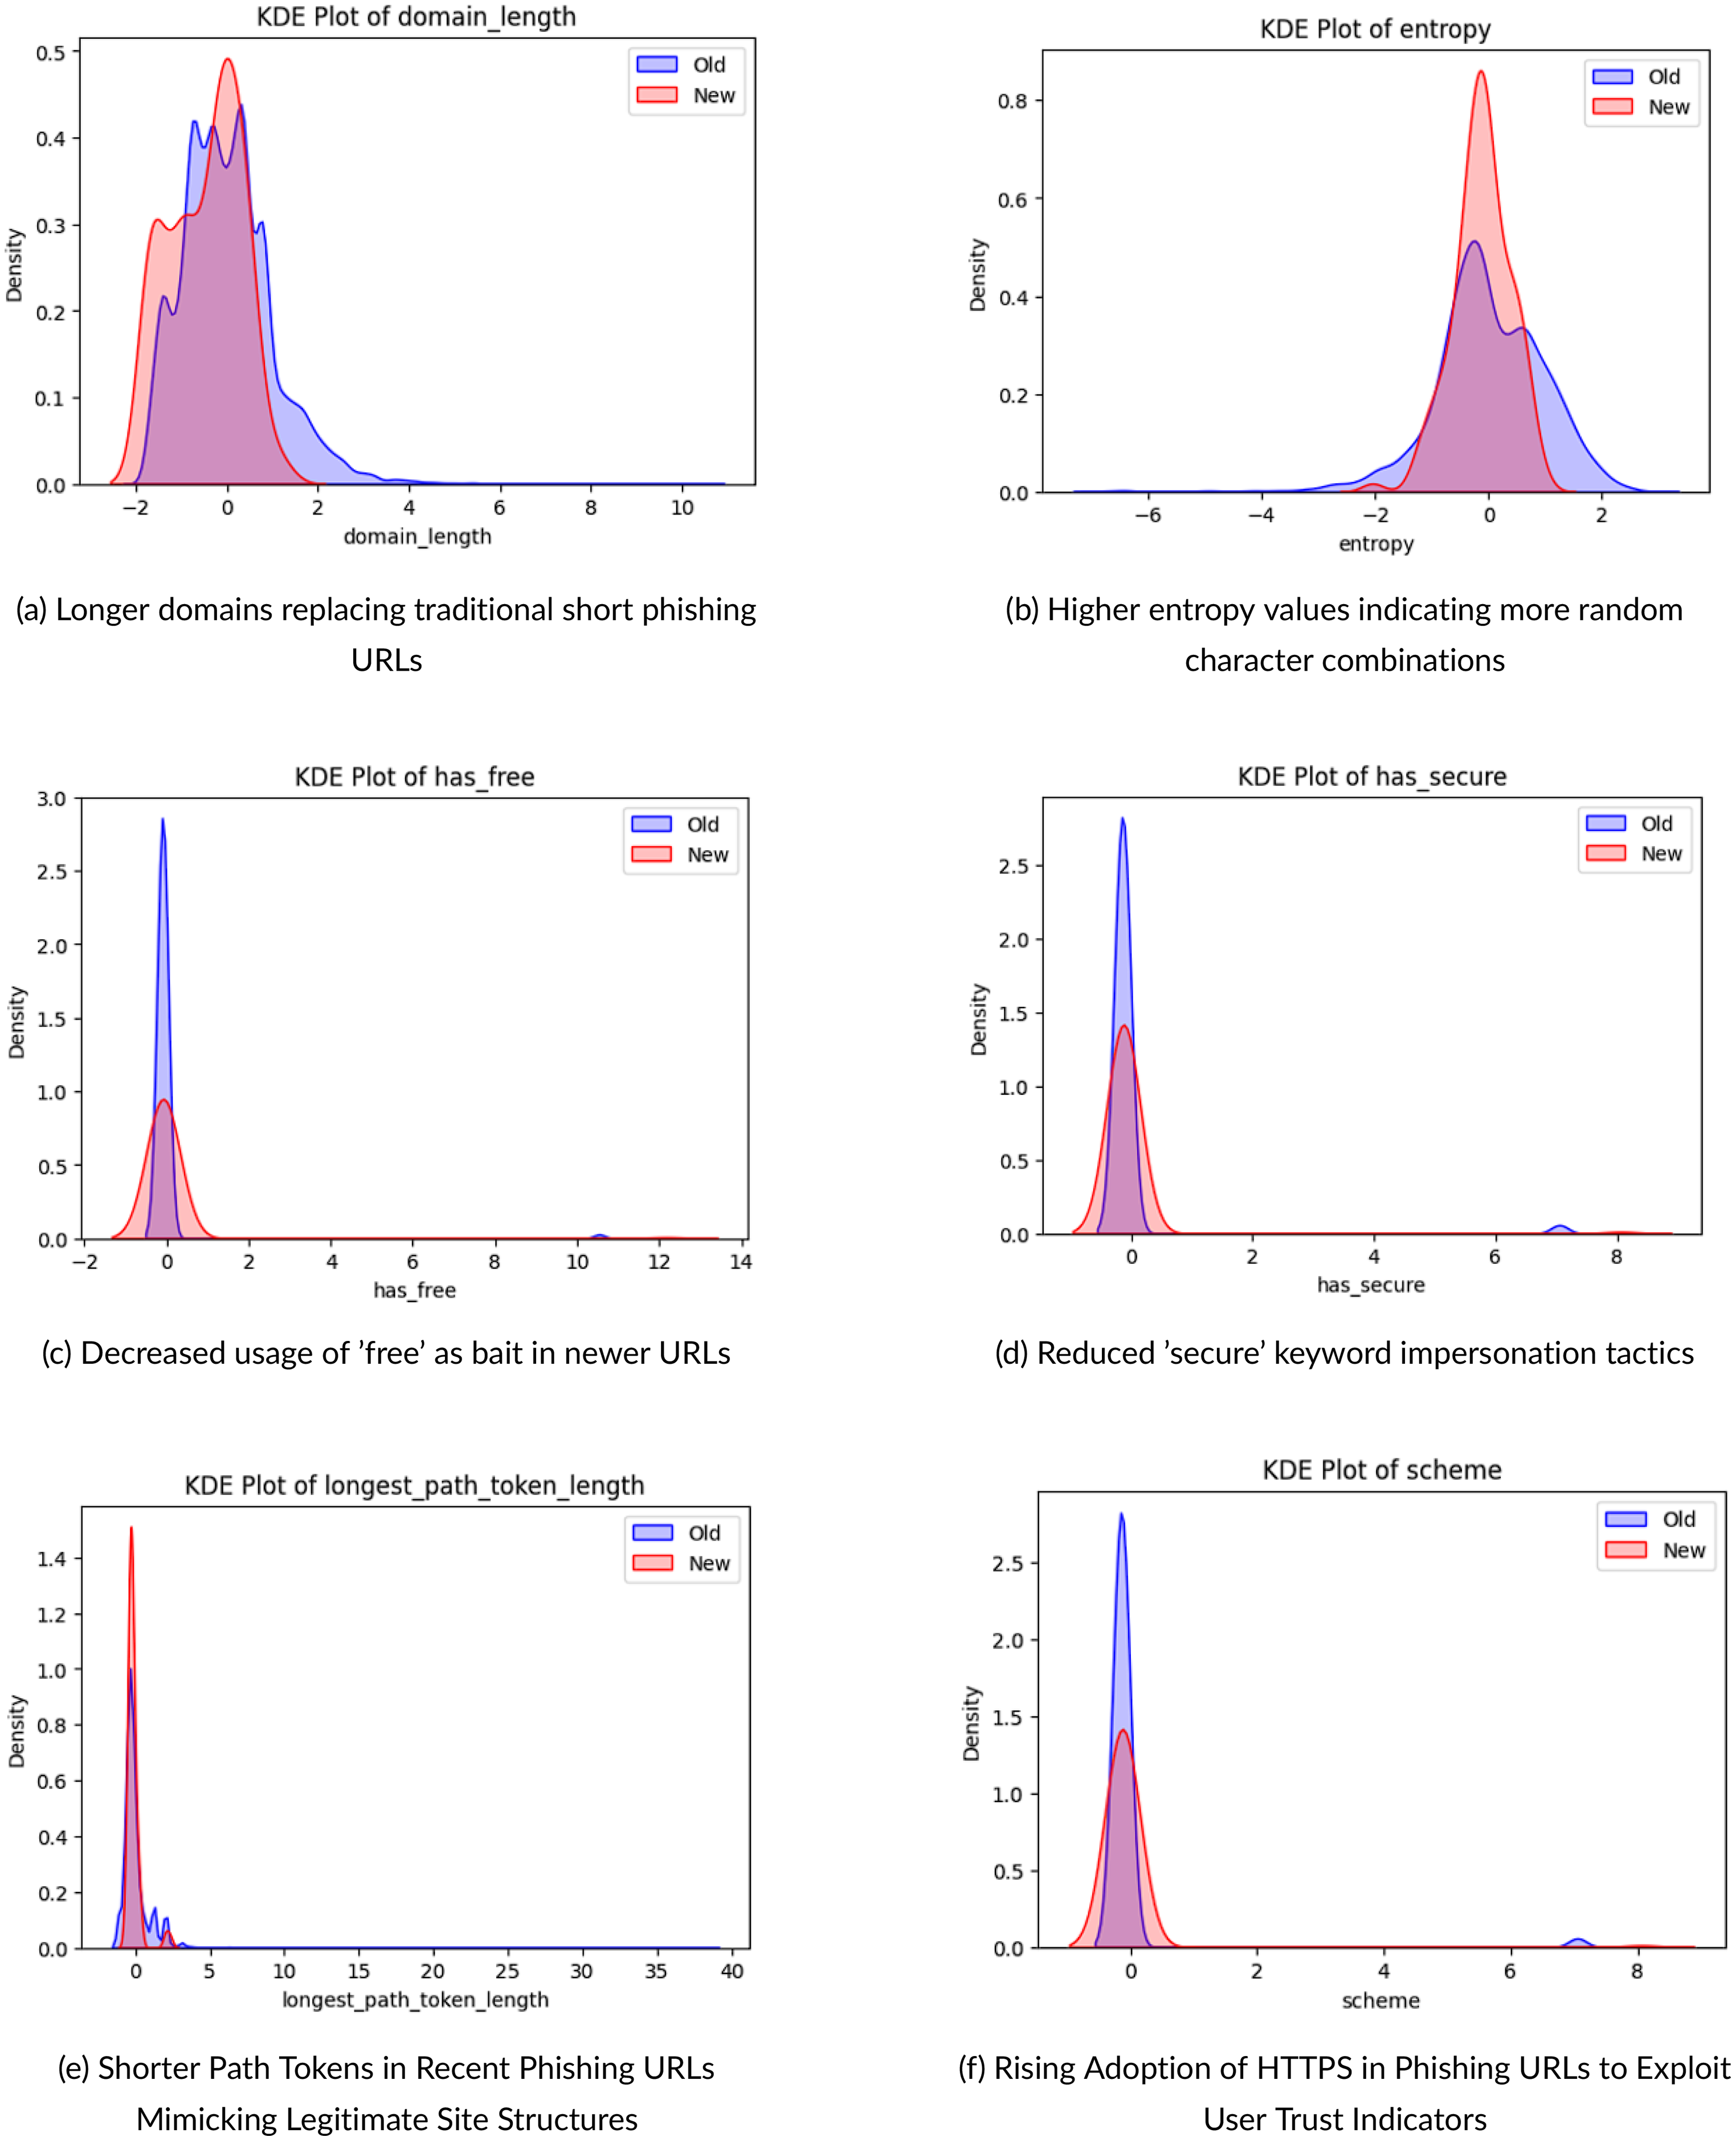
\includegraphics[height=0.62\textheight]{figures/paper_kde_a.png}
\end{column}
\begin{column}{0.38\textwidth}
  \centering
  {\scriptsize Ours (same features)}\\
  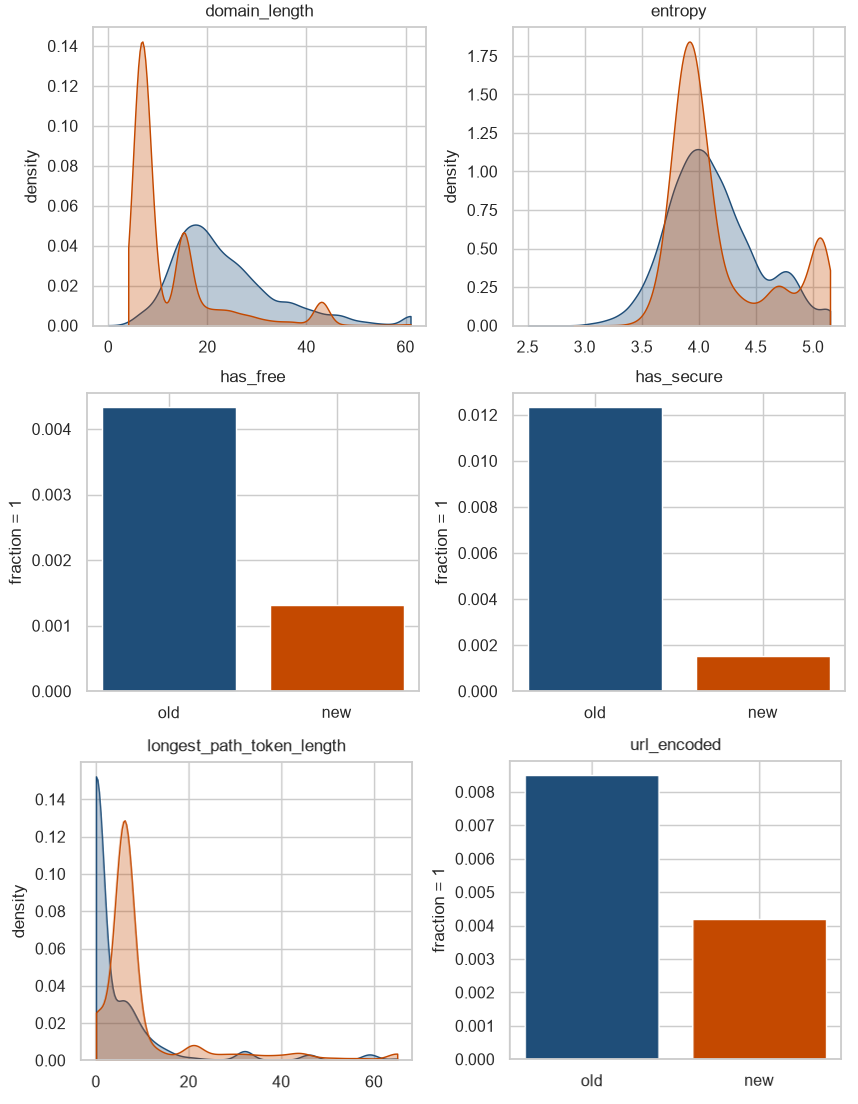
\includegraphics[height=0.62\textheight]{figures/ours_kde_6.png}
\end{column}
\begin{column}{0.22\textwidth}
  \begin{alertblock}{34 / 58}
  \scriptsize features differ (KS, $\delta{=}0.05$)
  \end{alertblock}
  \vspace{0.4em}
  \small New URLs: narrower ranges; bait words rarer. Paper premise holds on Jun\,2024--Jan\,2025 data.
\end{column}
\end{columns}
\end{frame}

% =============================================================================
\begin{frame}{KS statistic per feature (paper Fig.\,7)}
\begin{columns}[T,onlytextwidth]
\begin{column}{0.48\textwidth}
  \centering
  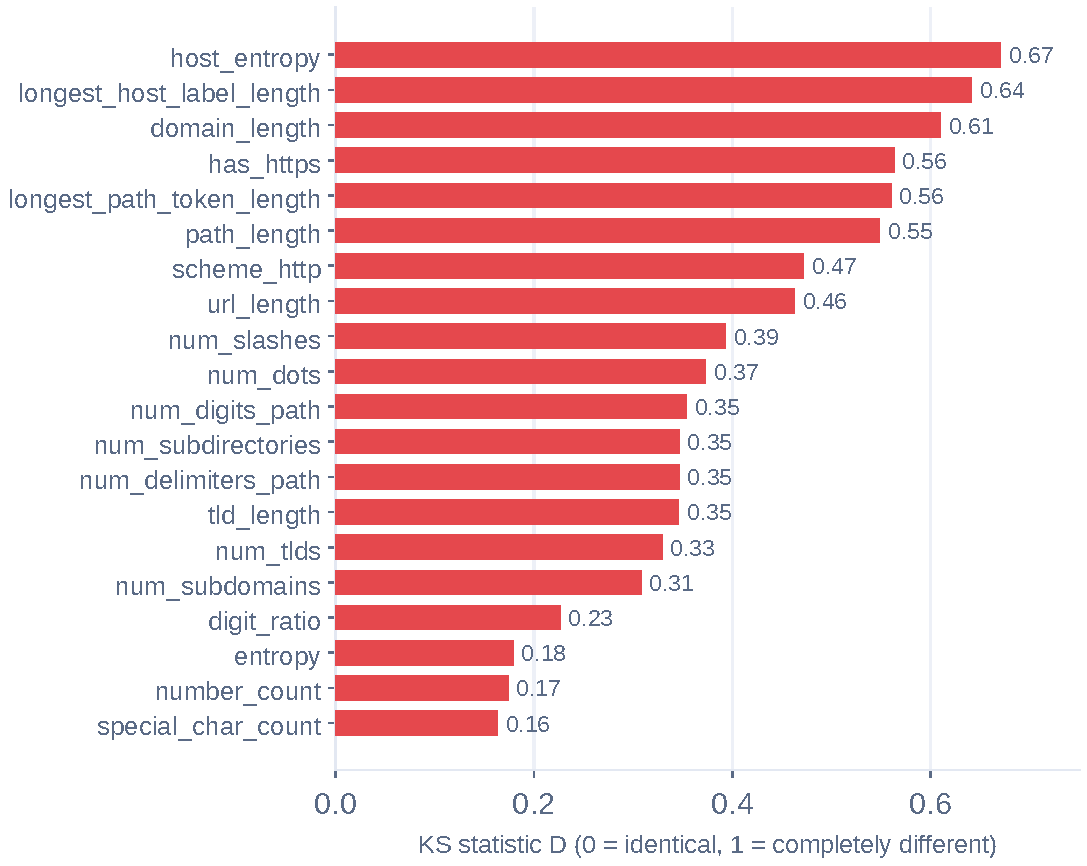
\includegraphics[height=0.68\textheight]{figures/c_ks_bars.pdf}
\end{column}
\begin{column}{0.49\textwidth}
  \centering
  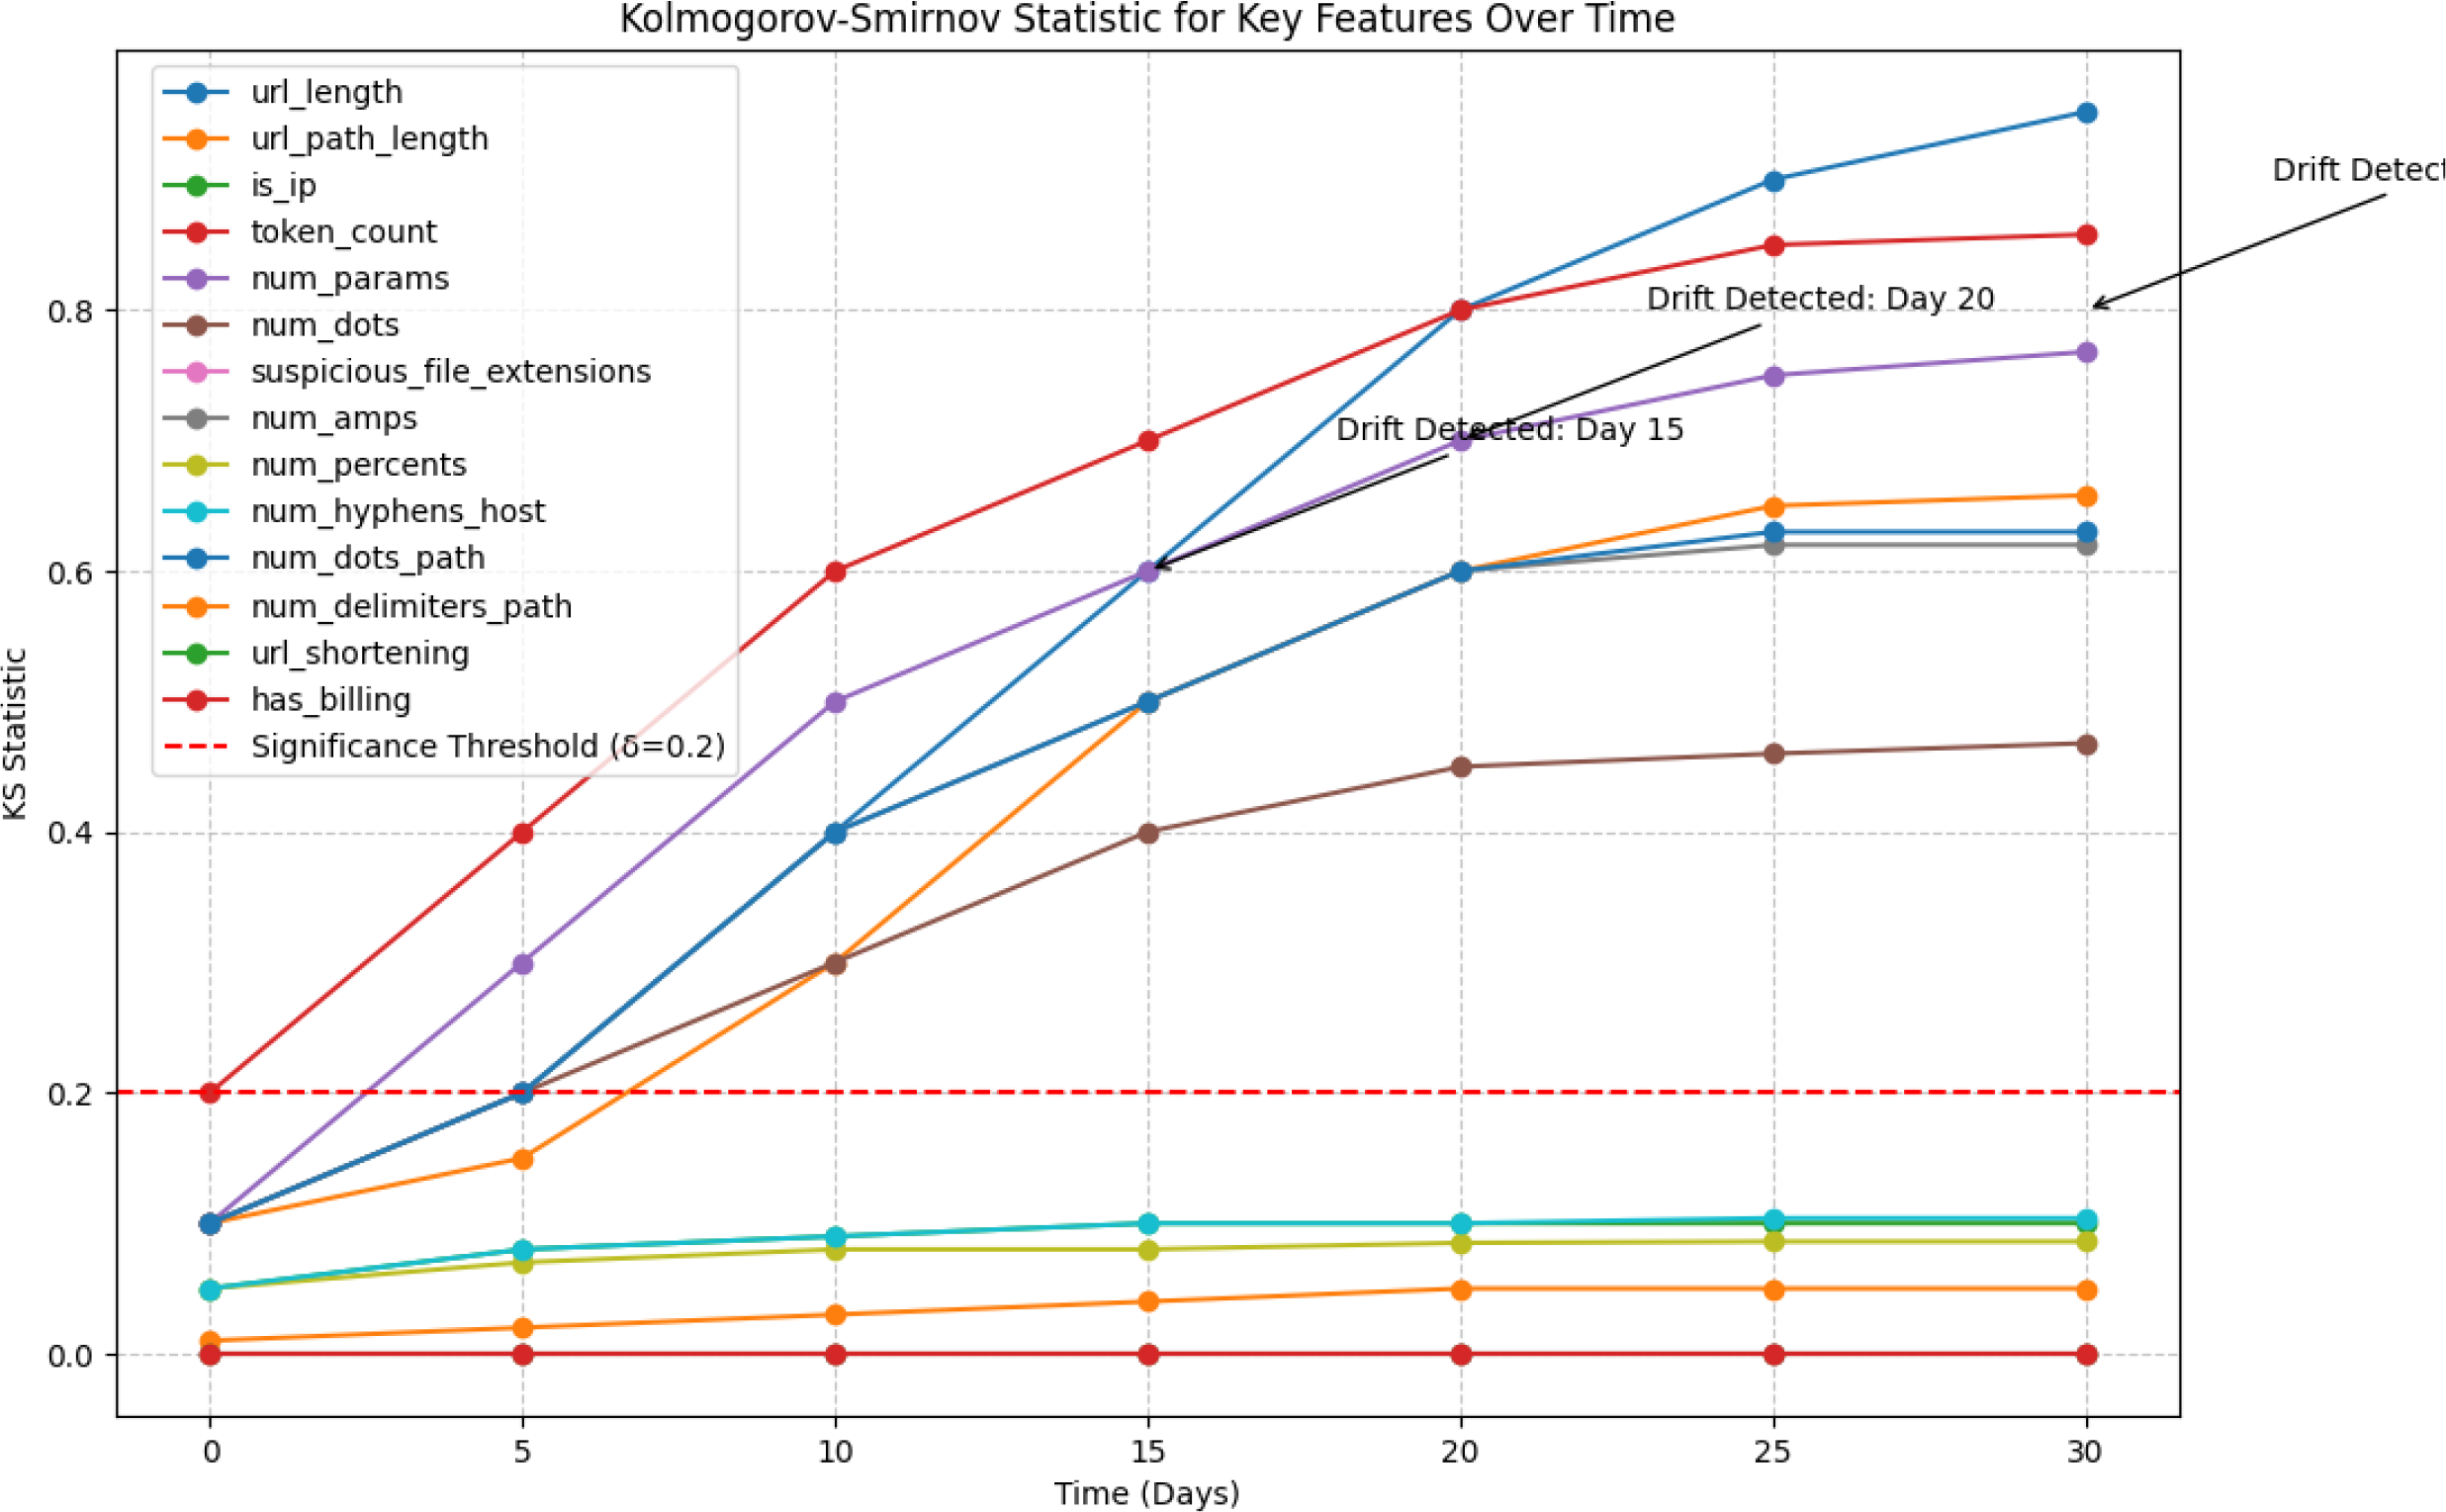
\includegraphics[width=\linewidth]{figures/paper_fig7_ks.png}\\[0.3em]
  \begin{block}{Reading it}
  \small Longer bar = bigger shift. Biggest: host entropy, host/domain length, https/http, path \& URL length --- length/structure family, as in the paper.
  \end{block}
\end{column}
\end{columns}
\end{frame}

% =============================================================================
\begin{frame}{Selected features change after drift (paper Table 8)}
\small
\begin{columns}[T,onlytextwidth]
\begin{column}{0.24\textwidth}
  \begin{block}{Initial}
  \scriptsize length, structure, https/http, digit\_ratio, \ldots
  \end{block}
\end{column}
\begin{column}{0.24\textwidth}
  \begin{alertblock}{Stage 1}
  \scriptsize +entropy, host\_entropy, longest\_host\_label\\
  $-$has\_https, num\_dots, scheme\_http
  \end{alertblock}
\end{column}
\begin{column}{0.24\textwidth}
  \begin{alertblock}{Stage 2}
  \scriptsize +num\_ampersand\\
  $-$num\_hyphens
  \end{alertblock}
\end{column}
\begin{column}{0.24\textwidth}
  \begin{alertblock}{Stage 3}
  \scriptsize +num\_digits\_query\\
  $-$num\_ampersand
  \end{alertblock}
\end{column}
\end{columns}
\vspace{0.55em}
\begin{exampleblock}{What this shows}
Feature set moves toward \textbf{host-name randomness} and \textbf{query-string} clues --- matching the paper's story that newer phishing relies on query obfuscation.
\hfill \pill{S1: 28.6 drift events} \pill{S2: 7 events}
\end{exampleblock}
\end{frame}

% =============================================================================
\begin{frame}{Results 3 --- Stream S1: online beats frozen by +5 pts}
\begin{columns}[T,onlytextwidth]
\begin{column}{0.62\textwidth}
  \centering
  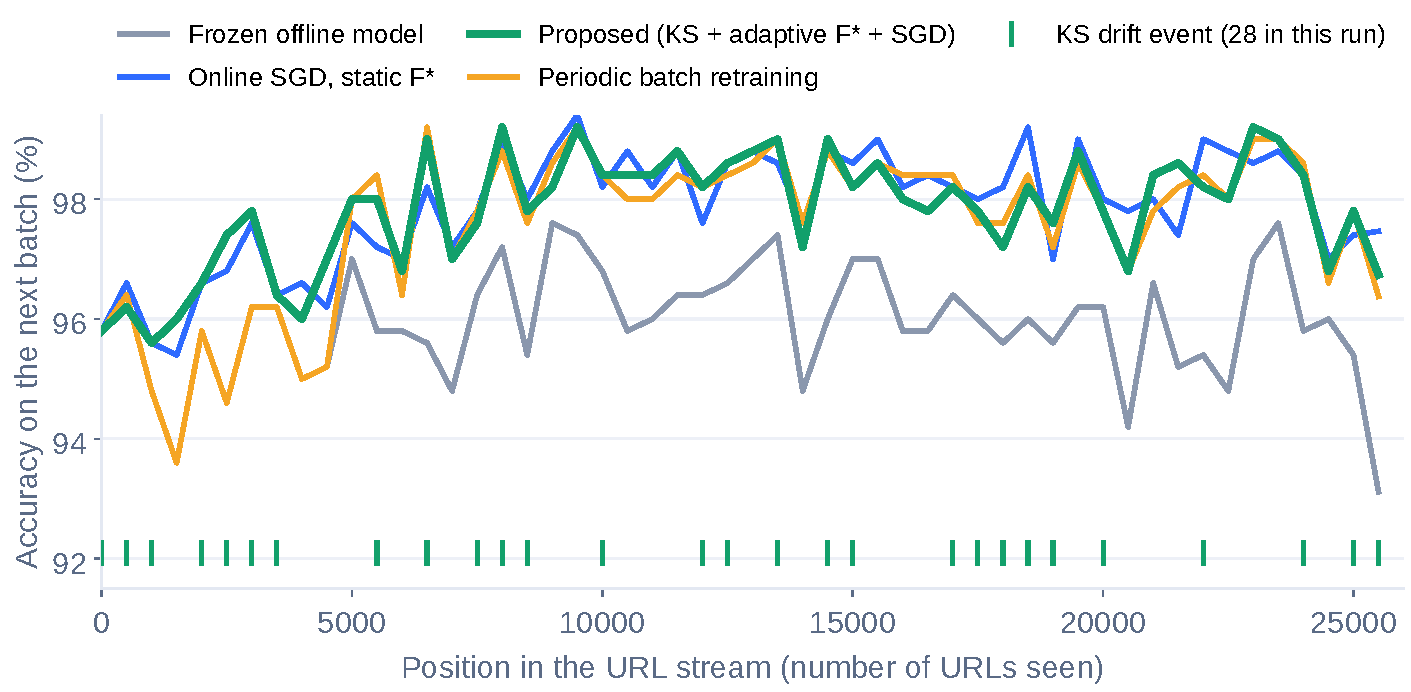
\includegraphics[width=\linewidth]{figures/c_stream_s1.pdf}\\[0.15em]
  \capnote{Prequential accuracy, 25{,}776 URLs (PhishTank window). Green ticks = KS events.}
\end{column}
\begin{column}{0.35\textwidth}
  \kpi[Muted]{Frozen}{92.63\%}\\[0.25em]
  \kpi{Online static $F^*$}{97.77\%}\\[0.25em]
  \kpi[Good]{Proposed adaptive}{97.80\%}\\[0.25em]
  \kpi[Warn]{Periodic batch}{97.31\%}
\end{column}
\end{columns}
\vspace{0.25em}
{\small \textcolor{Good}{\textbf{+5.1 pts}} over frozen, much lower variance ($\pm$0.05 vs $\pm$6.4).
Adaptive $\approx$ static here --- shift is gentle.}
\end{frame}

% =============================================================================
\begin{frame}{Stream S2 --- under big shifts, adaptive selection helps}
\begin{columns}[T,onlytextwidth]
\begin{column}{0.62\textwidth}
  \centering
  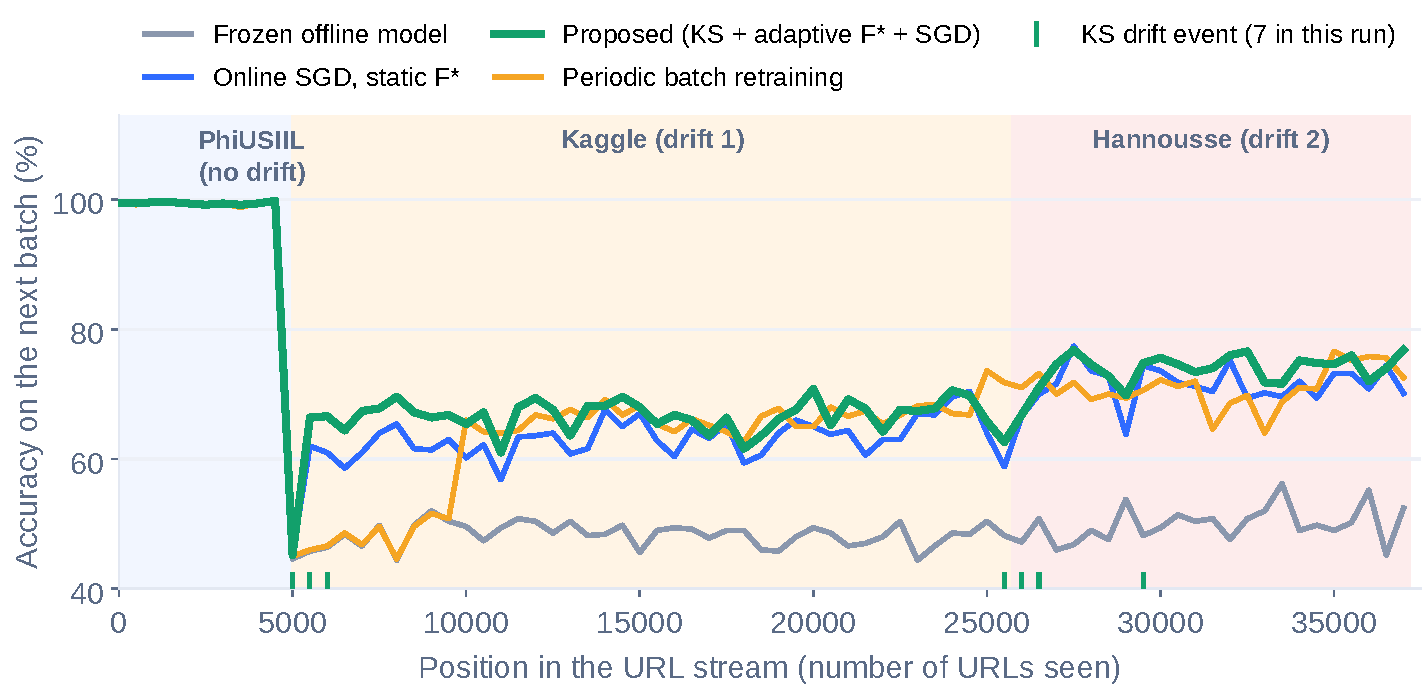
\includegraphics[width=\linewidth]{figures/c_stream_s2.pdf}\\[0.15em]
  \capnote{PhiUSIIL $\to$ Kaggle $\to$ Hannousse. Shading = corpus; ticks = drift events.}
\end{column}
\begin{column}{0.35\textwidth}
  \kpi[Muted]{Frozen}{55.5\%}\\[0.25em]
  \kpi{Online static}{70.5\%}\\[0.25em]
  \kpi[Good]{Proposed adaptive}{73.2\%}\\[0.25em]
  \kpi[Warn]{Periodic batch}{70.0\%}
\end{column}
\end{columns}
\vspace{0.25em}
{\small Adaptive gains \textbf{+2.7 pts} over static online --- feature re-selection matters when the distribution jumps hard.}
\end{frame}

% =============================================================================
\begin{frame}{Ablation (Table 9) --- when adaptive $F^*$ helps}
\begin{columns}[T,onlytextwidth]
\begin{column}{0.48\textwidth}
  \centering
  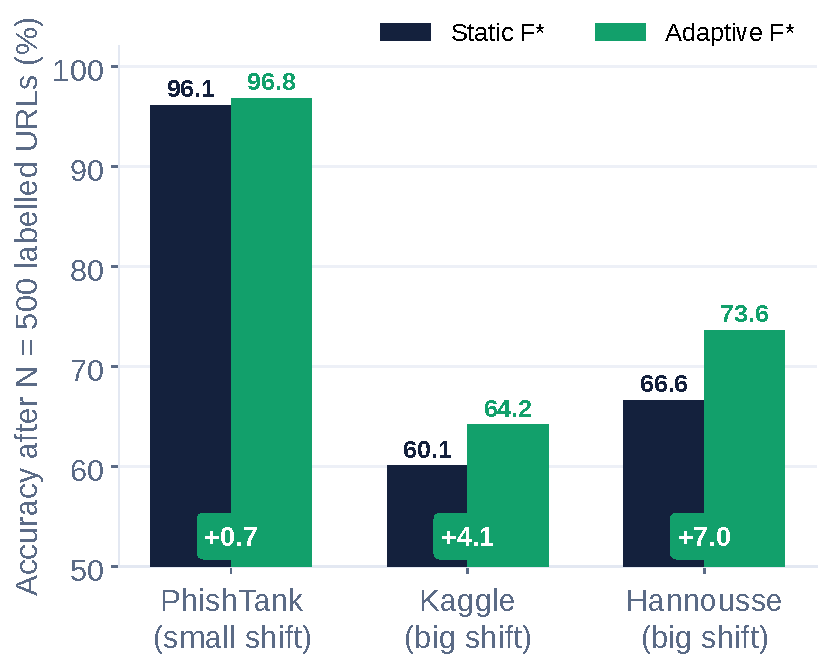
\includegraphics[width=\linewidth]{figures/c_ablation_acc.pdf}\\[0.1em]
  \capnote{Accuracy vs.\ \# new labelled URLs $N$.}
\end{column}
\begin{column}{0.48\textwidth}
  \centering
  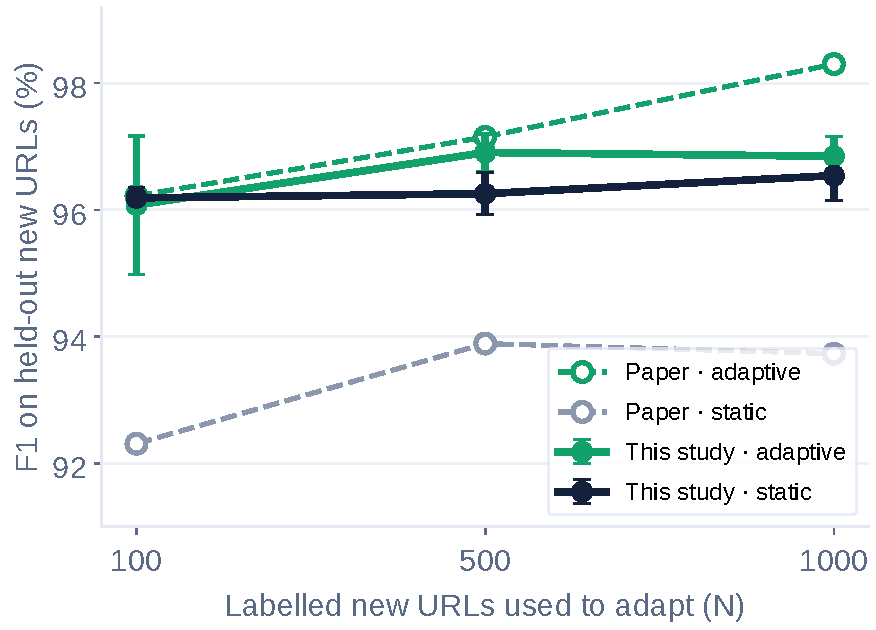
\includegraphics[width=\linewidth]{figures/c_ablation_f1.pdf}\\[0.1em]
  \capnote{F1; gains clearest on hard targets (Kaggle / Hannousse).}
\end{column}
\end{columns}
\vspace{0.25em}
{\small PhishTank (mild): adaptive $\approx$ static at high accuracy.
Hard shift: adaptive lifts accuracy and lowers FPR for $N\ge 500$.
Caveat: our static baseline is stronger than the paper's.}
\end{frame}

% =============================================================================
\begin{frame}{Runtime --- real-time scoring, cheap updates}
\begin{columns}[T,onlytextwidth]
\begin{column}{0.48\textwidth}
  \centering
  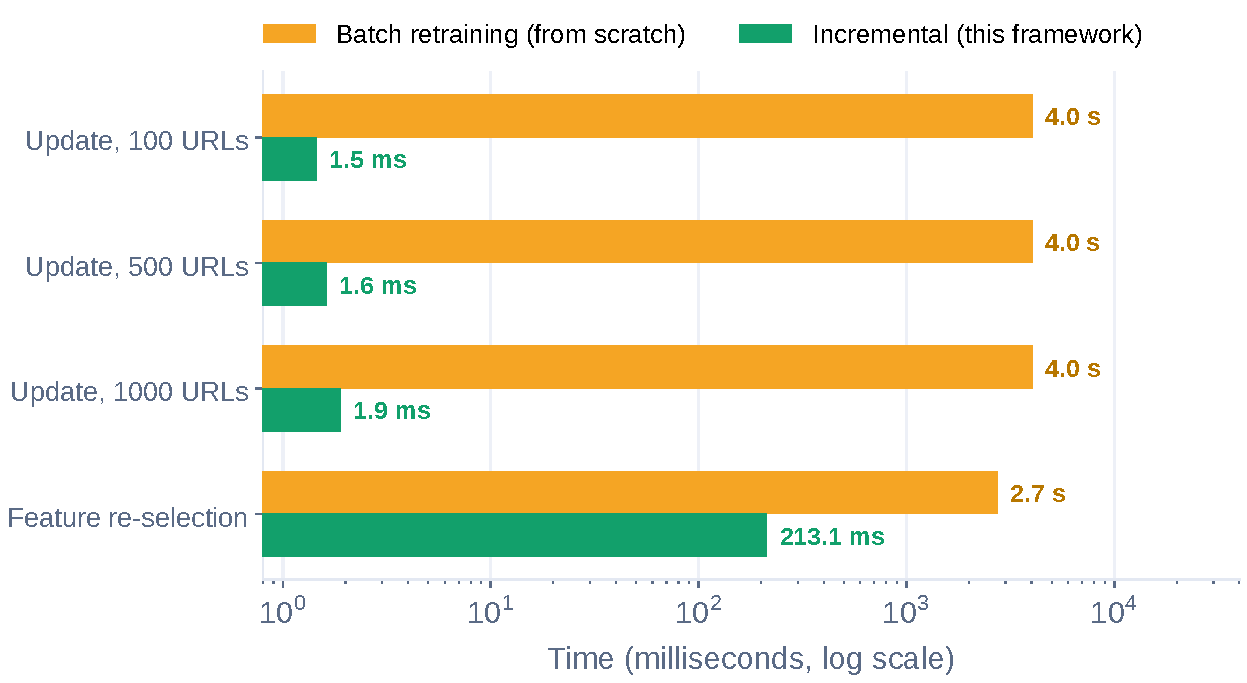
\includegraphics[width=\linewidth]{figures/c_runtime.pdf}
\end{column}
\begin{column}{0.49\textwidth}
  \begin{exampleblock}{Per-URL latency}
  \centering\textbf{0.16\,ms} avg (1 CPU thread)\\
  {\scriptsize Paper: 12.4--15.2\,ms (different HW)}
  \end{exampleblock}
  \vspace{0.4em}
  {\footnotesize
  \begin{tabular}{@{}lrrr@{}}
  \toprule
  Op & Incr. & Batch & Gain \\
  \midrule
  Update 100 & 1.5\,ms & 4.0\,s & $\mathbf{2770\times}$ \\
  Update 500 & 1.6\,ms & 4.0\,s & $2477\times$ \\
  Update 1k & 1.9\,ms & 4.0\,s & $2140\times$ \\
  Feat.\ adapt & 213\,ms & 2.7\,s & $13\times$ \\
  \bottomrule
  \end{tabular}}
\end{column}
\end{columns}
\end{frame}

% =============================================================================
\begin{frame}{Scorecard --- what reproduced vs.\ what is lower-level}
\renewcommand{\arraystretch}{1.18}
{\footnotesize
\begin{tabular}{@{}p{0.42\linewidth}p{0.24\linewidth}p{0.24\linewidth}@{}}
\toprule
Claim / experiment & Ours & Verdict \\
\midrule
PhiUSIIL SGD-SVM accuracy & 99.38\% (paper 98.78) & \textcolor{Good}{\textbf{matches}} \\
SVM best of 3 SGD variants & yes & \textcolor{Good}{\textbf{matches}} \\
Old vs new distributions drift & 34/58 features & \textcolor{Good}{\textbf{matches}} \\
$F^*$ changes after drift (T8) & logged swaps & \textcolor{Good}{\textbf{matches}} \\
Online $>$ frozen (streams) & +5.1 / +15.0 pts & \textcolor{Good}{\textbf{matches}} \\
Ablation adaptive F1 (PhishTank) & $\approx$ paper & \textcolor{Good}{\textbf{close}} \\
ISCX / Kaggle / Combined absolute & lower & \textcolor{Warn}{\textbf{ordering OK}} \\
Incremental $\gg$ batch cost & $10^3\times$ & \textcolor{Good}{\textbf{same conclusion}} \\
\bottomrule
\end{tabular}}
\vspace{0.45em}
\tagline{We reproduce the \textbf{method behaviour} and qualitative claims.
Absolute levels on some corpora depend on unpublished feature defs / data versions.}
\end{frame}

% =============================================================================
\begin{frame}{Demo --- PhishCheck (browser, lexical SGD-SVM)}
\begin{columns}[T,onlytextwidth]
\begin{column}{0.32\textwidth}
  \centering
  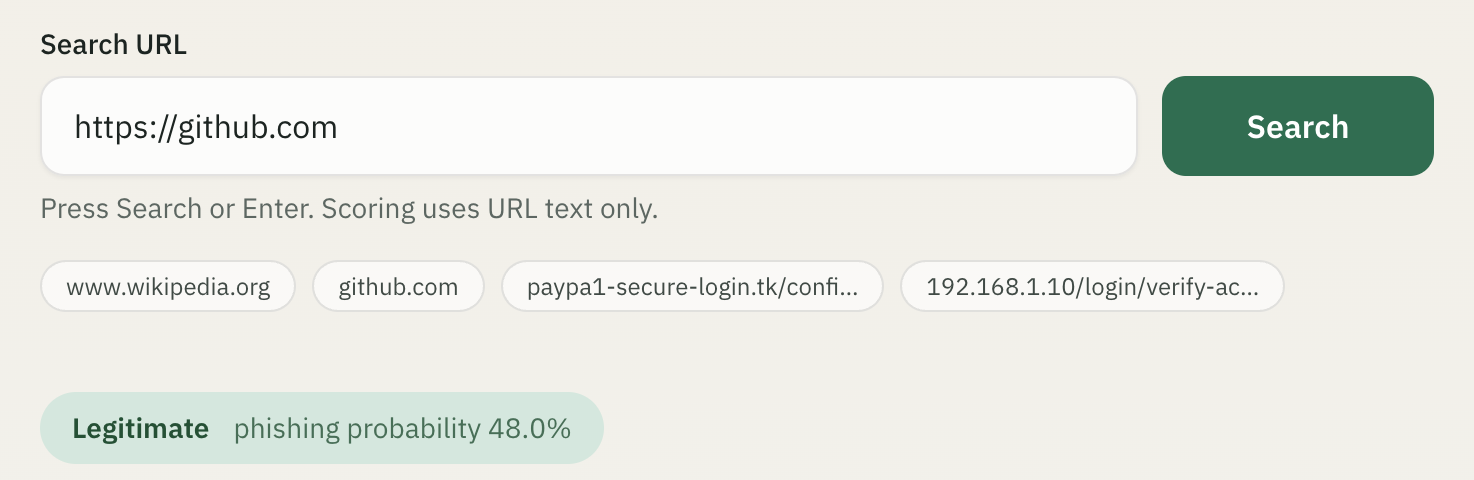
\includegraphics[width=\linewidth]{figures/demo_legit.png}\\
  \capnote{Clean legit URL}
\end{column}
\begin{column}{0.32\textwidth}
  \centering
  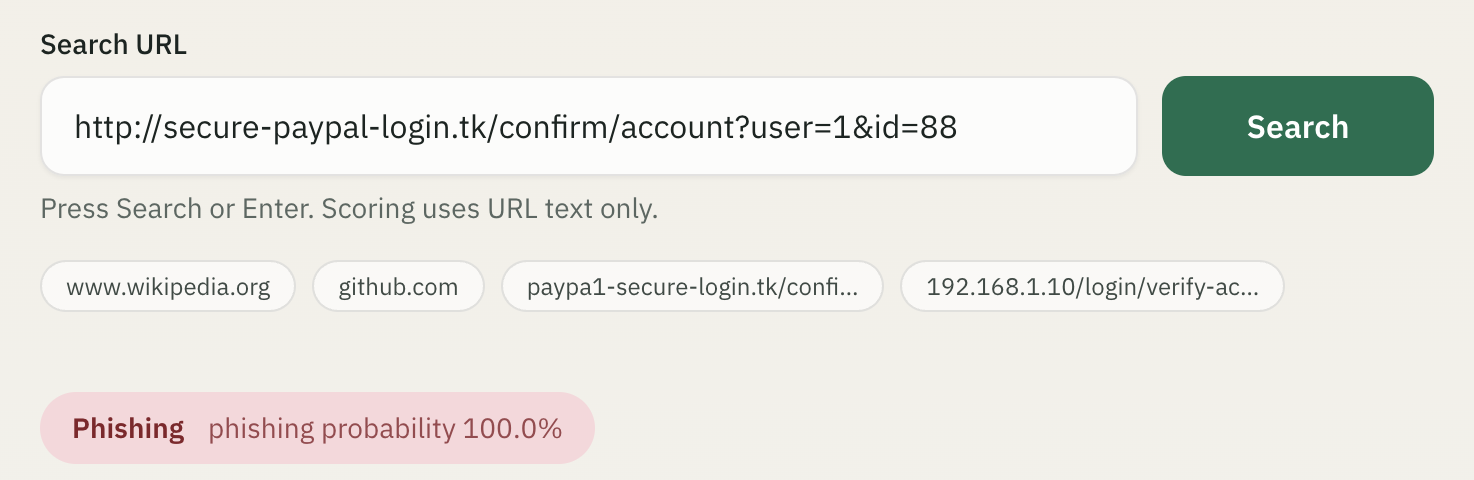
\includegraphics[width=\linewidth]{figures/demo_phish.png}\\
  \capnote{Obvious phishing URL}
\end{column}
\begin{column}{0.32\textwidth}
  \centering
  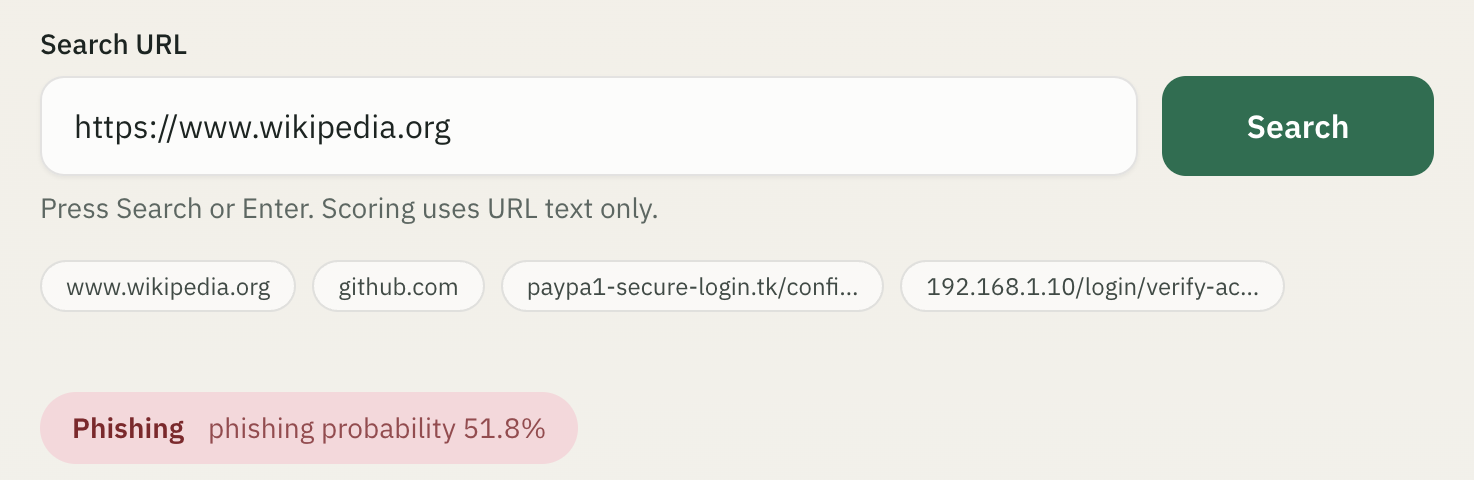
\includegraphics[width=\linewidth]{figures/demo_wiki.png}\\
  \capnote{Bare domain near boundary}
\end{column}
\end{columns}
\vspace{0.35em}
\begin{alertblock}{Limitation (be upfront)}
\small URL-only models can false-alarm on bare domains with little context
(e.g.\ \texttt{wikipedia.org} near the decision boundary). Live demo:
\texttt{Source\_Code/web/}.
\end{alertblock}
\end{frame}

% =============================================================================
\begin{frame}{Takeaways}
\begin{columns}[T,onlytextwidth]
\begin{column}{0.48\textwidth}
  \begin{exampleblock}{What we learned}
  \begin{itemize}
    \item URL lexical features + online SGD work in real time
    \item Concept drift is measurable (34/58 features)
    \item Online learning recovers +5 to +15 pts vs frozen
    \item Adaptive $F^*$ helps most under \textbf{strong} shifts
  \end{itemize}
  \end{exampleblock}
\end{column}
\begin{column}{0.48\textwidth}
  \begin{alertblock}{Limitations \& next}
  \begin{itemize}
    \item Absolute levels need paper's exact features / cleaning
    \item No HTML / third-party signals (by design)
    \item Drift-event rule (25\%) is our design choice
    \item Future: richer features, better bare-domain handling
  \end{itemize}
  \end{alertblock}
\end{column}
\end{columns}
\vspace{0.55em}
\tagline{Reproduce everything: \texttt{cd Source\_Code \&\& make all}
\quad·\quad Report: \texttt{Project\_Report.pdf}
\quad·\quad Results: \texttt{Experimental\_Results/RESULTS.md}}
\end{frame}

% =============================================================================
\begin{frame}[plain]
\begin{tikzpicture}[remember picture,overlay]
  \fill[Navy] (current page.south west) rectangle (current page.north east);
\end{tikzpicture}
\vspace*{2.2em}
\begin{center}
  {\Huge\bfseries\color{white} Questions?\par}
  \vspace{0.9em}
  {\large\color{AccentSoft} Thank you\par}
  \vspace{1.4em}
  {\normalsize\color{white} Pratham Garg · Sumit Sharma · Vivaan Garg\par}
  \vspace{0.5em}
  {\small\color{AccentSoft} CS\,552 · Krishnan \& Naik, \emph{Security and Privacy} 2025\par}
  \vspace{0.35em}
  {\footnotesize\color{AccentSoft} DOI 10.1002/spy2.70057\par}
\end{center}
\end{frame}

% =============================================================================
\appendix
\begin{frame}{Appendix A --- Combined SGD-SVM vs paper Fig.\,6}
\centering
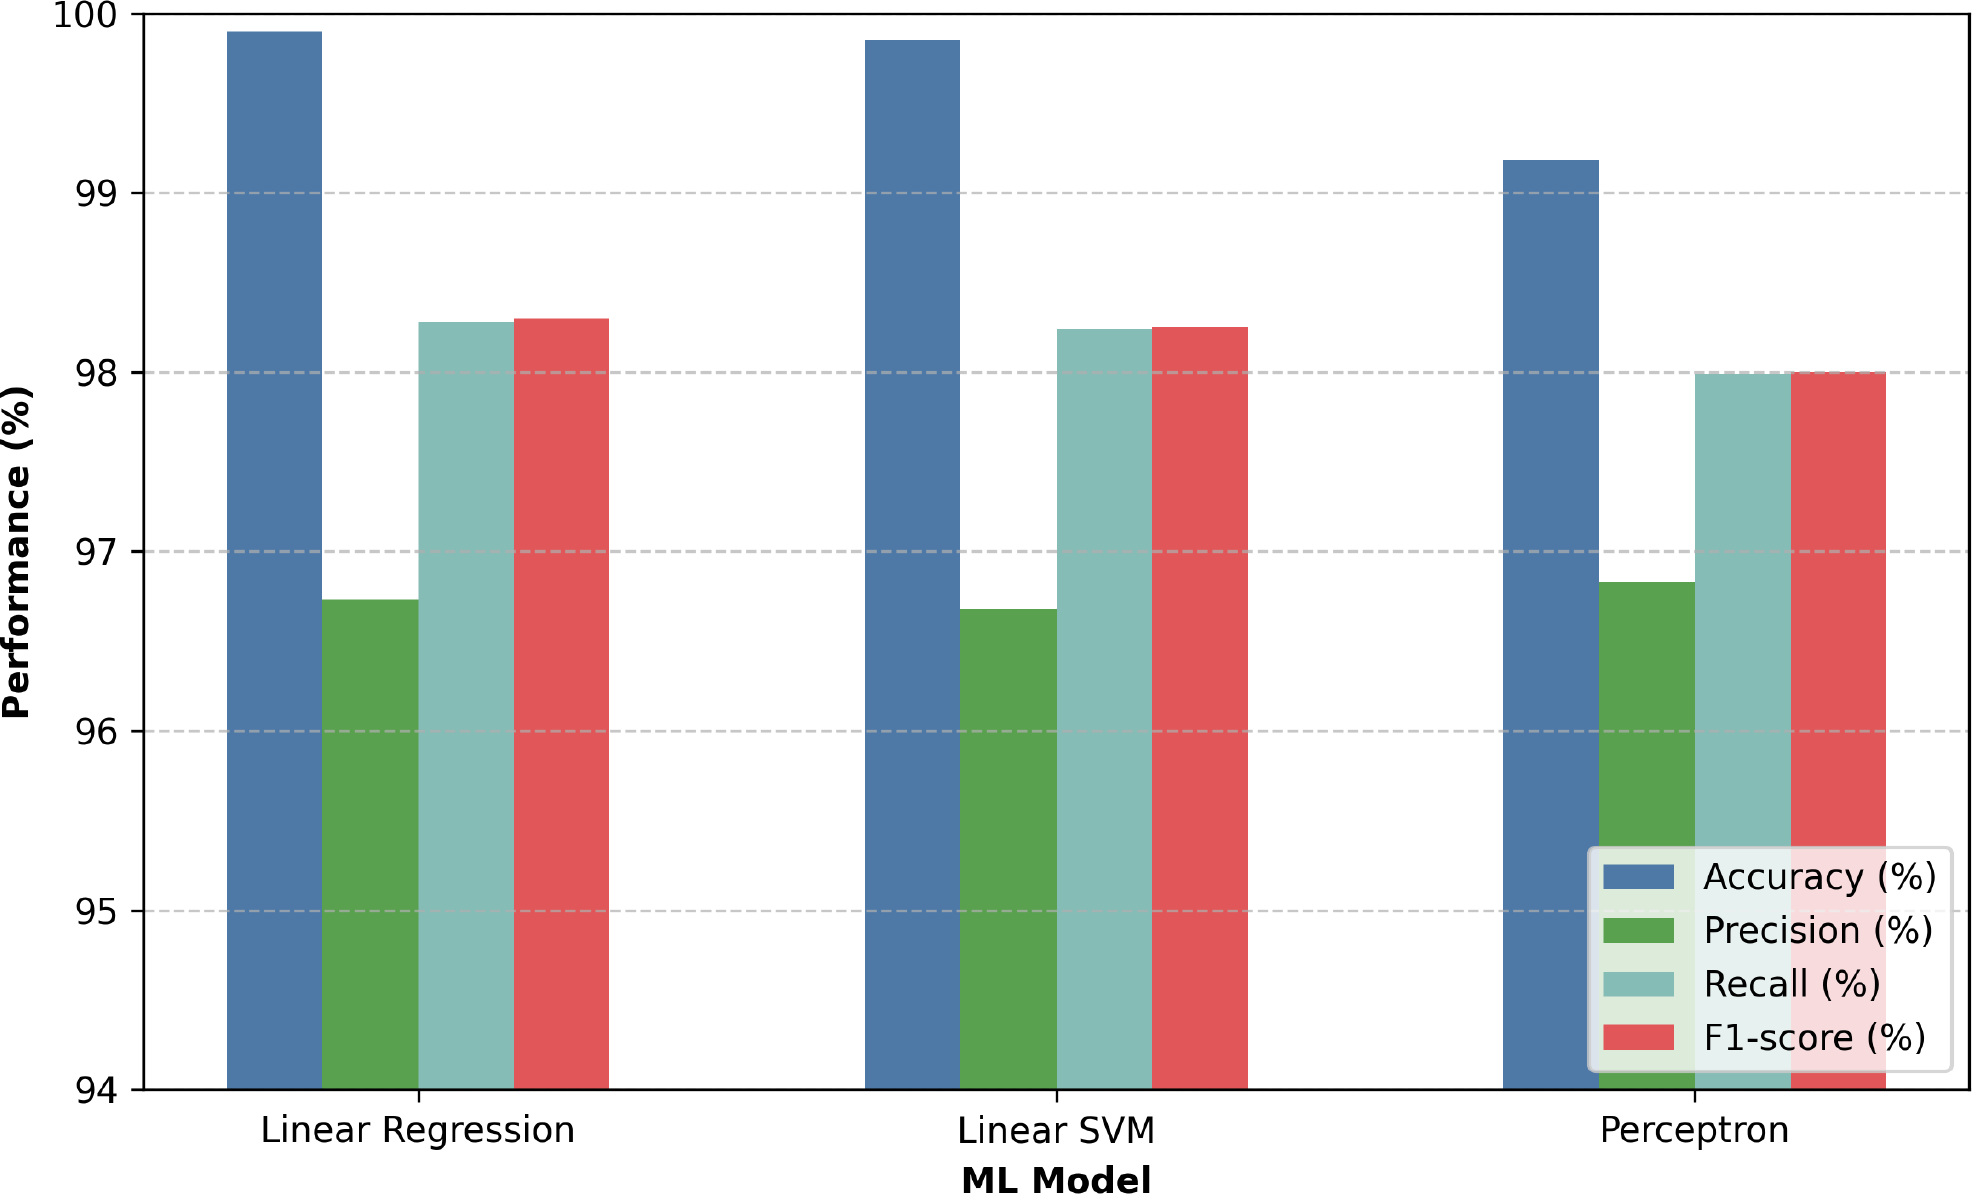
\includegraphics[width=0.72\linewidth]{figures/paper_fig6_perf.png}\\[0.3em]
\capnote{Paper Fig.\,6. Our combined SGD-SVM: 93.58\% acc, 6.23\% FPR (same ordering of SGD variants).}
\end{frame}

\begin{frame}{Appendix B --- Feature co-occurrence (paper Fig.\,5)}
\begin{columns}[T,onlytextwidth]
\begin{column}{0.48\textwidth}
  \centering{\scriptsize Paper}\\
  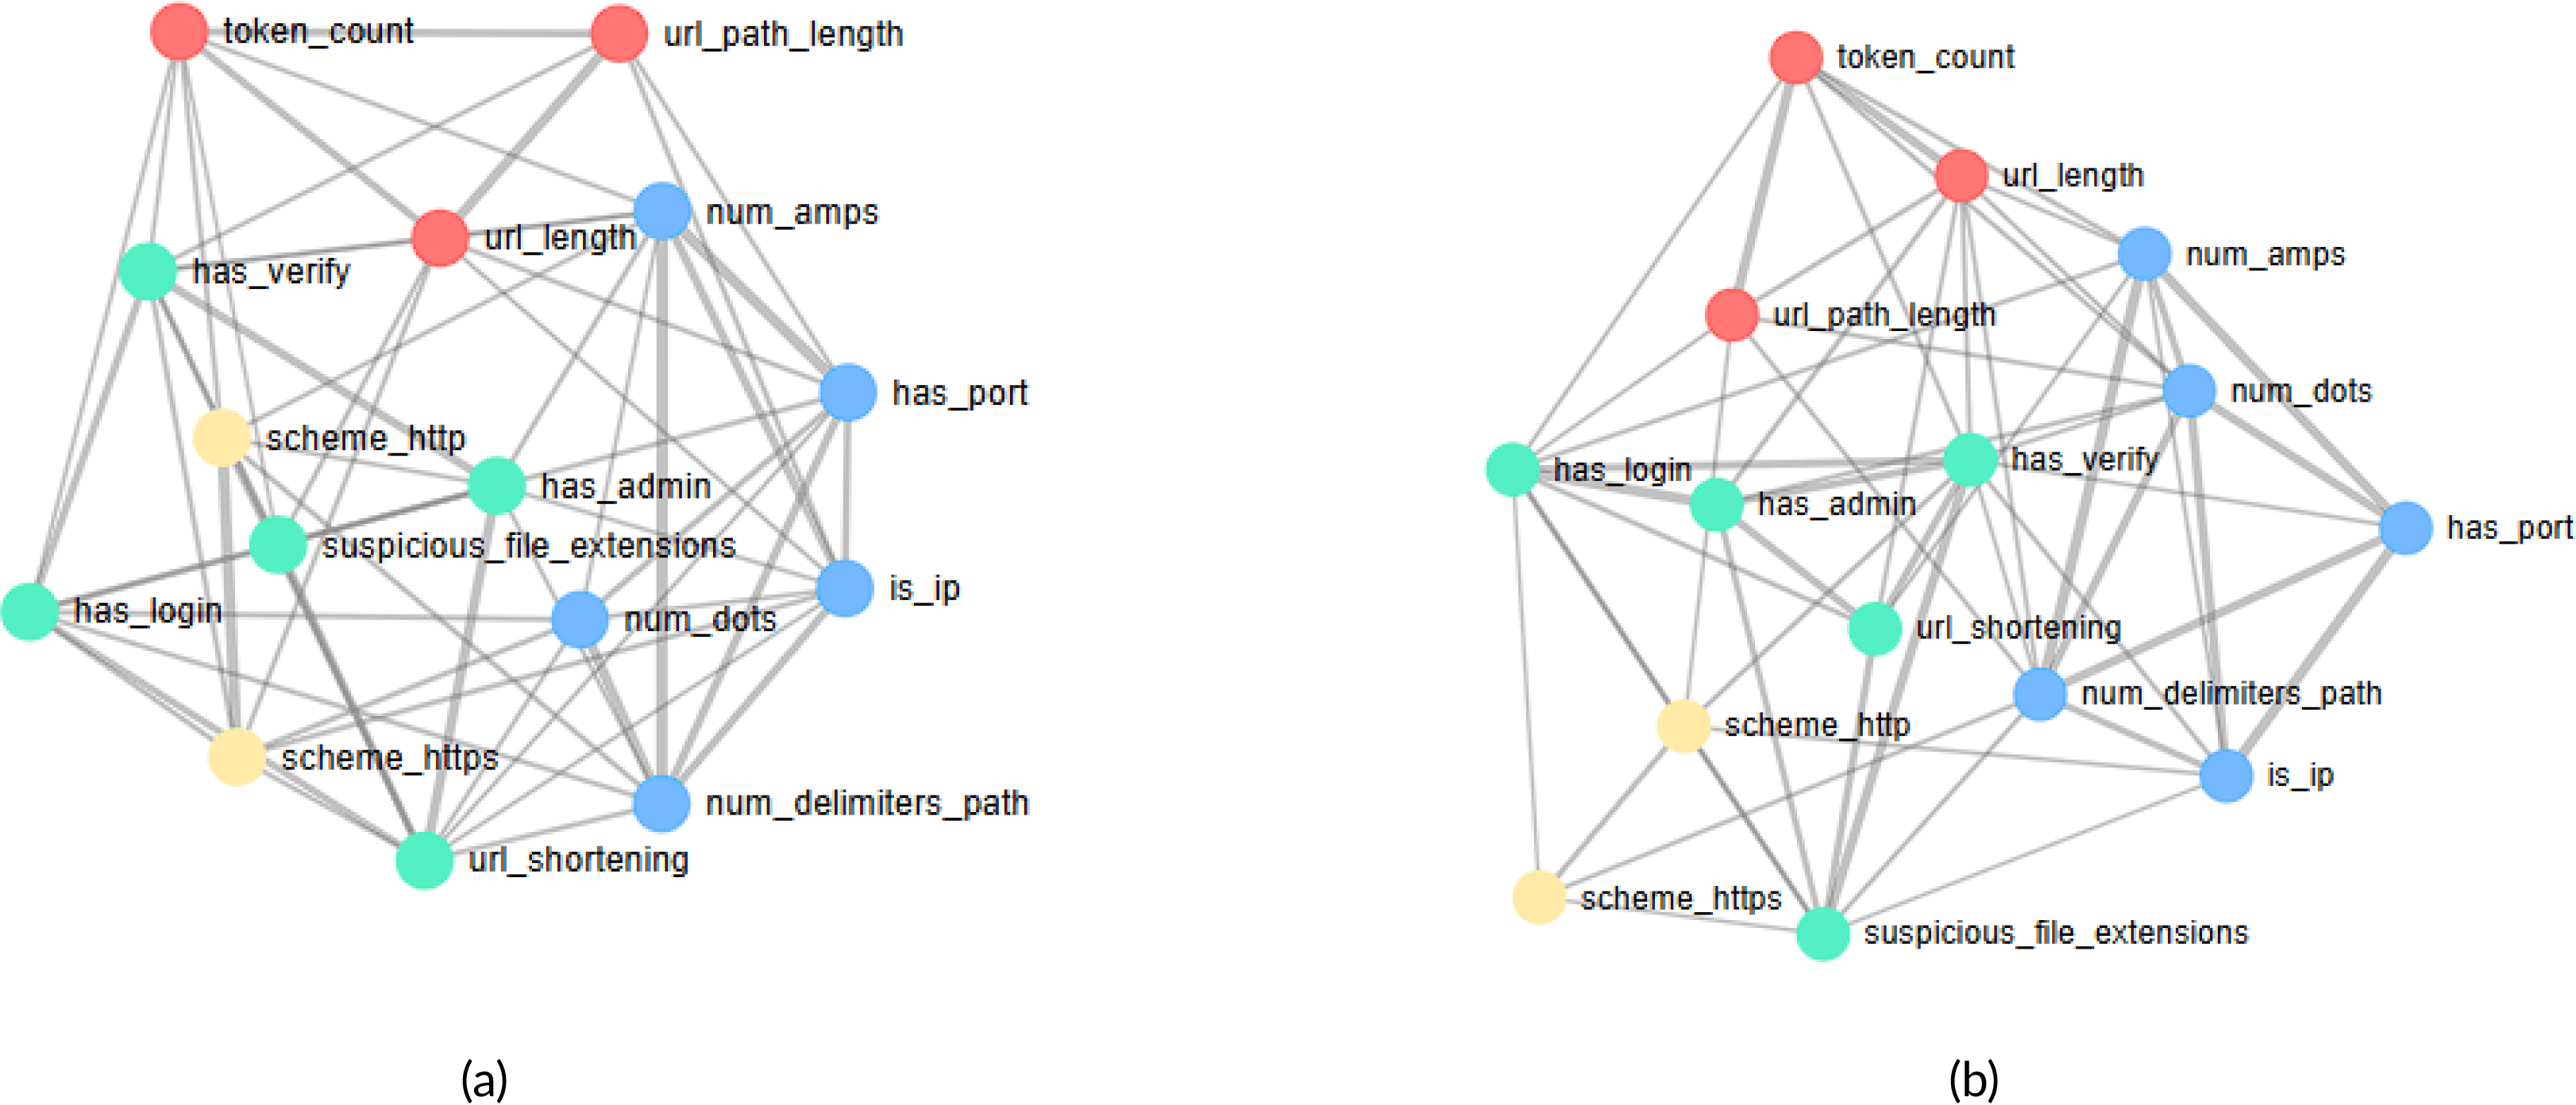
\includegraphics[width=\linewidth]{figures/paper_fig5_cooc.png}
\end{column}
\begin{column}{0.48\textwidth}
  \centering{\scriptsize Ours}\\
  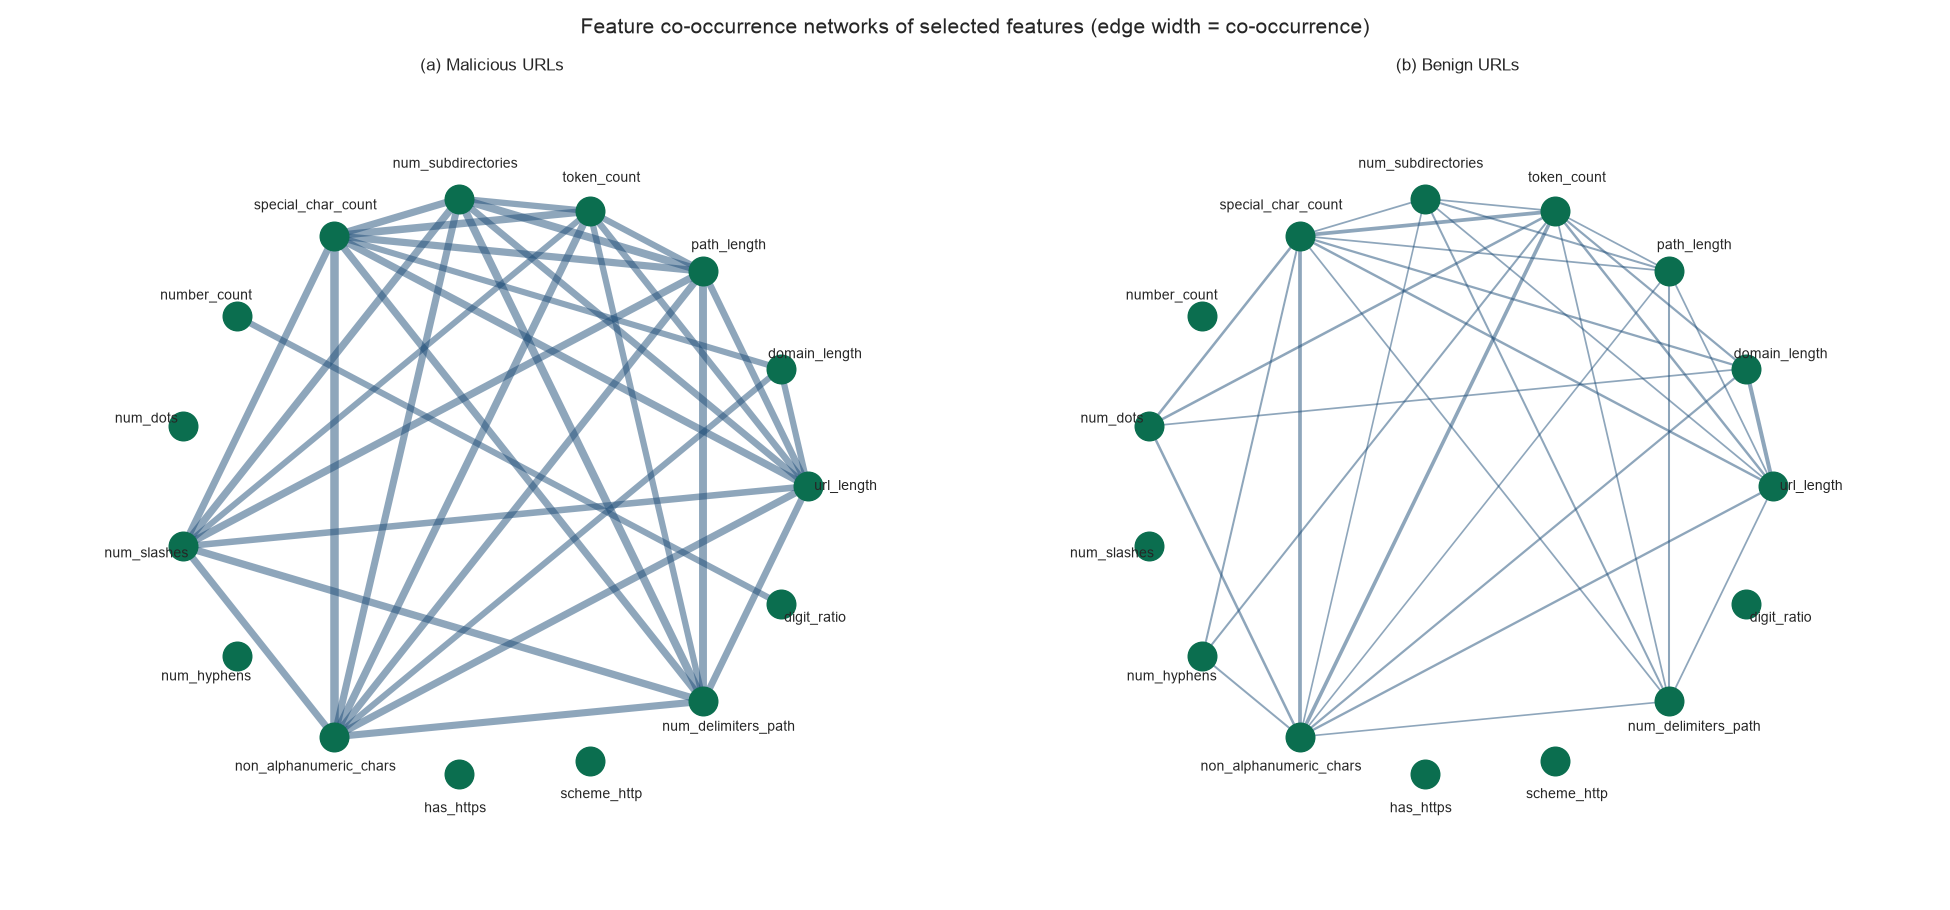
\includegraphics[width=\linewidth]{figures/ours_fig5_cooccurrence.png}
\end{column}
\end{columns}
\end{frame}

\begin{frame}{Appendix C --- Stream bars (S1 vs S2 summary)}
\centering
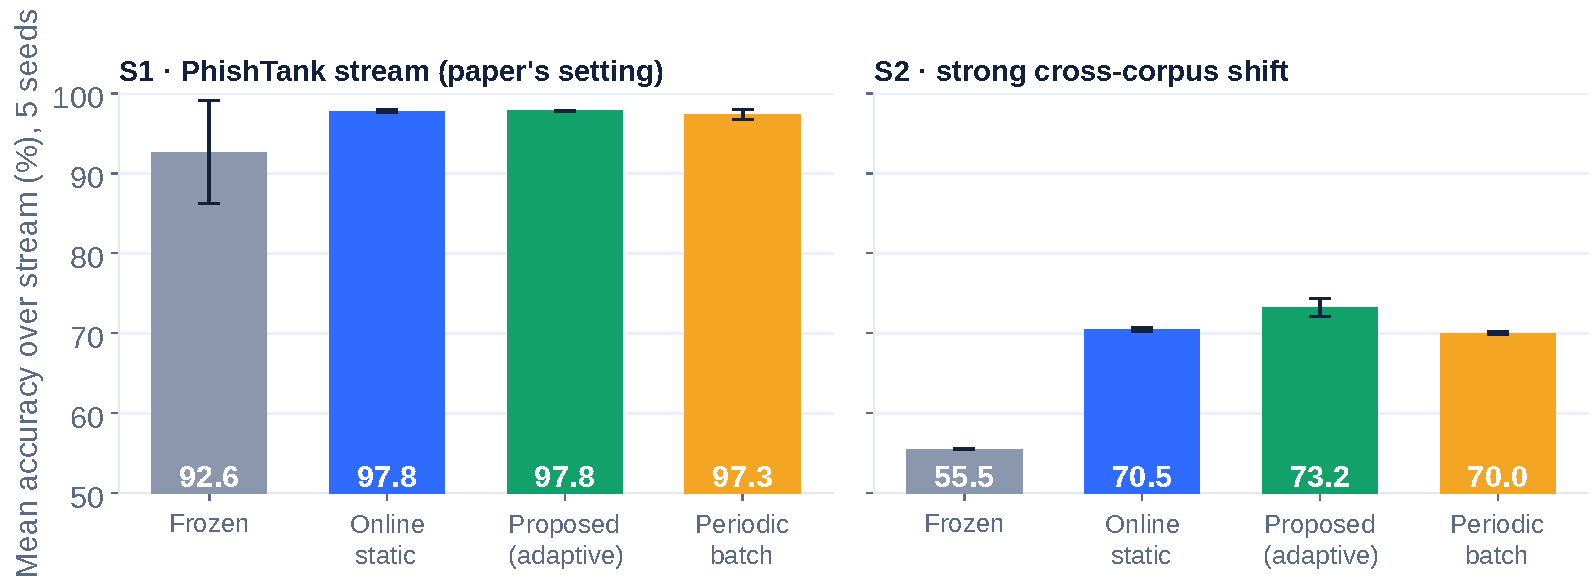
\includegraphics[width=0.85\linewidth]{figures/c_stream_bars.pdf}
\end{frame}

\end{document}
